\chapter{Results} \label{sec:results}
\epigraph{Great quote.}{Author}
\begin{figure}[H]
	\centering
	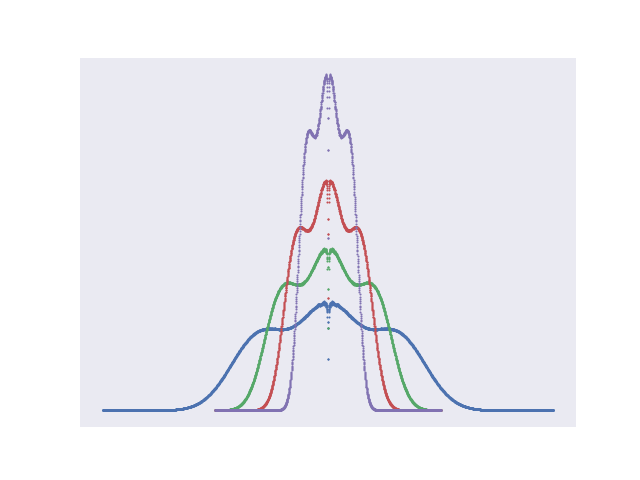
\includegraphics[scale=0.7]{Images/art.png}
	\caption{One-body density plots for a two-dimensional single quantum dot containing 12 electrons, popularly called an artificial Magnesium atom. The four graphs correspond to four different oscillator frequencies, where the weakest oscillator gives the broadest density distribution. It's quite artistic, isn't it?}
\end{figure}
After all, this thesis is related to a master in physics, and therefore the results and the physical insight is the interesting part. Before we move on to the physical results, we will take a quick look at some more technical results, more precisely the computational cost of various wave function structures and the energy convergence using various optimization tools. 

For validation purposes, we will present a few selected results on the case without repulsive interaction and compare to analytical results. Thereafter, we study the case with repulsive interaction in a much larger scale, where we compare various wave function structures for different number of particles and oscillator strengths in two and three dimensions.

\newpage
\section{Computational cost}
One of the major problems when performing quantum many-body simulations is the computational cost, which explodes as the system size increases. In figure \eqref{fig:cpu_time} the CPU-time is plotted as a function of the number of particles. We observe that the restricted Boltzmann machine (RBM) generally is cheaper to calculate compared to standard variational Monte-Carlo (VMC), which is a bit surprising. In the VMC trial wave function, we have only two variational parameters, while in the RBM we have $N\cdot D\cdot (1+H)+H$ with $N$ as number of particles $D$ as the number of dimensions and $H$ as the number of hidden nodes. Throughout this thesis we always set $H=N$, which was found to give the lowest energies when testing on small systems. \cite{nordhagen_computational_2018} 

With our choice of hidden nodes, we end up with 10,584 parameters for 72 particles in two dimensions and 14,980 parameters for 70 particles in three dimensions. In other words, this evolve to be an optimization problem. The reason why the RBM still appears to have a cheaper cost, is probably that we do not need to calculate the distance matrix over and over again, and the very efficient LAPACK and BLAS packages lie behind the matrix operations. For RBM+SJ and RBM+PJ, the cost is significantly higher because of the update of the distance matrix.

\iffalse
\begin{figure} %[h]
	\centering
	% This file was created by matplotlib2tikz v0.7.4.
\begin{tikzpicture}[scale=0.9]

\begin{axis}[name=2D, xlabel=$N$, ylabel={CPU-time [s]}, grid=major, 
legend cell align={left},
legend style={at={(1.68,1.10)}, anchor=south east, draw=white!80.0!black},
legend columns = 6, 
clip=false,
xtick=data] 
\addplot[color=color0,mark=oplus*, dashed] coordinates { 
	(2,6.05)
	(6,11.25)
	(12,20.53) 
	(20,38.99) 
	(30,73.73) 
	(42,130.49) 
	(56,213.47)
	(72,360.22)
	(90,856.84) }; 
\addlegendentry{RBM};

\addplot[color=color1,mark=oplus*, dash dot] coordinates { 
	(2,7.12) 
	(6,14.07) 
	(12,28.42) 
	(20,63.27) 
	(30,122.93) 
	(42,199.60)
	(56,349.22)}; 
\addlegendentry{RBM+SJ};

\addplot[color=color2,mark=oplus*, dotted] coordinates { 
	(2,7.26)
	(6,13.50)
	(12,27.68)
	(20,57.09) 
	(30,119.17) 
	(42,212.53) 
	(56,382.13) }; 
\addlegendentry{RBM+PJ};

\addplot[color=color3,mark=oplus*] coordinates { 
	(2,5.11)
	(6,10.51)
	(12,20.85) 
	(20,41.20) 
	(30,76.26) 
	(42,137.39) 
	(56,230.63)
	(72,355.81)
	(90,544.03) }; 
\addlegendentry{VMC};

\node[] at (axis cs: 44,978) {2D};
\end{axis}

\begin{axis}[name=2D, 
xshift=7.9cm, 
xlabel=$N$, 
grid=major, 
clip=false,
xtick=data] 
\addplot[color=color0,mark=oplus*, dashed] coordinates { 
	(2,7.69)
	(8,20.92)
	(20,59.67) 
	(40,171.84) 
	(70,586.39) }; 
%\addlegendentry{RBM};

\addplot[color=color1,mark=oplus*, dash dot] coordinates { 
	(2,8.95)
	(8,26.86)
	(20,94.64) 
	(40,270.92) }; 
%\addlegendentry{RBM+SJ};

\addplot[color=color2,mark=oplus*, dotted] coordinates { 
	(2,8.87)
	(8,26.36)
	(20,91.40) 
	(40,293.25) }; 
%\addlegendentry{RBM+PJ};

\addplot[color=color3,mark=oplus*] coordinates { 
	(2,6.70)
	(8,20.99)
	(20,62.54) 
	(40,185.65) 
	(70,486.02) };
%\addlegendentry{VMC};

\node[] at (axis cs: 35,670) {3D};
\end{axis}
\end{tikzpicture}
	\caption{CPU-time per iteration as a function of number of particles for two and three dimensions. The solid line is standard variational Monte-Carlo (VMC), while the dashed lines are restricted Boltzmann machines without Jastrow factor (RBM), with simple Jastrow factor (RBM+SJ) and with Padé-Jastrow factor (RBM+PJ).}
	\label{fig:cpu_time1}
\end{figure}
\fi

\begin{figure}
	\centering 
	\subfloat[2D]{{% This file was created by matplotlib2tikz v0.7.4.
\begin{tikzpicture}[scale=0.9]

\begin{axis}[name=2D, xlabel=$N$, ylabel={CPU-time [s]}, grid=major, legend pos=north west, xtick=data] 
\addplot[color=color1,mark=oplus*, dashed] coordinates { 
	(2,6.05)
	(6,11.25)
	(12,20.53) 
	(20,38.99) 
	(30,73.73) 
	(42,130.49) 
	(56,213.47)
	(72,360.22)
	(90,856.84) }; 
\addlegendentry{RBM};

\addplot[color=color2,mark=oplus*, dash dot] coordinates { 
	(2,7.12) 
	(6,14.07) 
	(12,28.42) 
	(20,63.27) 
	(30,122.93) 
	(42,199.60)
	(56,349.22)}; 
\addlegendentry{RBM+SJ};

\addplot[color=color3,mark=oplus*, dotted] coordinates { 
	(2,7.26)
	(6,13.50)
	(12,27.68)
	(20,57.09) 
	(30,119.17) 
	(42,212.53) 
	(56,382.13) }; 
\addlegendentry{RBM+PJ};

\addplot[color=color0,mark=oplus*] coordinates { 
	(2,5.11)
	(6,10.51)
	(12,20.85) 
	(20,41.20) 
	(30,76.26) 
	(42,137.39) 
	(56,230.63)
	(72,355.81)
	(90,544.03) }; 
\addlegendentry{VMC};
\end{axis}
\end{tikzpicture}}}
	\subfloat[3D]{{% This file was created by matplotlib2tikz v0.7.4.
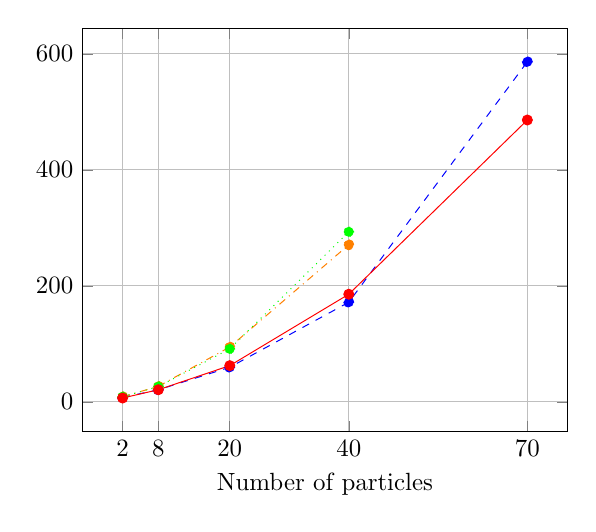
\begin{tikzpicture}[scale=0.9]

\definecolor{color0}{rgb}{0.12156862745098,0.466666666666667,0.705882352941177}
\definecolor{color1}{rgb}{1,0.498039215686275,0.0549019607843137}

\begin{axis}[name=2D, xlabel=Number of particles, grid=major, xtick=data] 
\addplot[color=blue,mark=oplus*, dashed] coordinates { 
	(2,7.69)
	(8,20.92)
	(20,59.67) 
	(40,171.84) 
	(70,586.39) }; 
%\addlegendentry{RBM};

\addplot[color=orange,mark=oplus*, dash dot] coordinates { 
	(2,8.95)
	(8,26.86)
	(20,94.64) 
	(40,270.92) }; 
%\addlegendentry{RBM+SJ};

\addplot[color=green,mark=oplus*, dotted] coordinates { 
	(2,8.87)
	(8,26.36)
	(20,91.40) 
	(40,293.25) }; 
%\addlegendentry{RBM+PJ};

\addplot[color=red,mark=oplus*] coordinates { 
	(2,6.70)
	(8,20.99)
	(20,62.54) 
	(40,185.65) 
	(70,486.02) };
%\addlegendentry{VMC};
\end{axis}

\end{tikzpicture}}}
	\caption{CPU-time per iteration as a function of number of particles for two dimensions (a) and three dimensions (b). The solid line is associated with standard variational Monte-Carlo (VMC), while the dashed lines are associated with restricted Boltzmann machines without Jastrow factor (RBM), with simple Jastrow factor (RBM+SJ) and with Padé-Jastrow factor (RBM+PJ).}
	\label{fig:cpu_time}
\end{figure} 

As the applied theory used in quantum many-body simulations agrees perfectly with laboratory experiments, they can be considered as actual experiments. In that manner, one can use computer experiments to verify other experiments and even predict new things. Similarly to experiments in a laboratory, computer experiments are also dependent on external factors, especially when it comes to the CPU-time, and therefore it is important to do such measurements multiple times to find an accurate average time. The CPU-times above are the average from at least four independent runs for each number of particles. All the runs were performed on the Abel computational cluster, which is equipped with Supermicro X9DRT compute nodes with dual Intel E5-2670 CPUs running at 2.6 GHz. Different hardware might give different CPU-times, but the CPU-time ratios (the exponential factor) should be the same. 

To estimate how fast the cost increases as we add more particles, we do linear regression with a function on the form $f(x)=\alpha x^{\beta}$ where $x$ is the number of particles while $\alpha$ and $\beta$ are the unknown parameters to be found. From the limited number of points, we have found the parameters and presented them in table \eqref{tab:cputimefit}. Although the RBM was found to be cheaper than VMC, we can see that the estimated exponential factor $\alpha$ is actually slightly larger. The prefactor $\beta$ is significantly lower though.

\begin{table}
	\caption{Optimal constants $\alpha$ and $\beta$ for restricted Boltzmann machine (RBM), restricted Boltzmann machine with a simple Jastrow factor (RBM+SJ), restricted Boltzmann machine with Padé-Jastrow factor (RBM+PJ) and standard variational Monte-Carlo sampling (VMC).}
	\begin{tabularx}{\textwidth}{X|CC:CC} \hline\hline
		\label{tab:cputimefit}
		& \multicolumn{2}{c}{2D} &
		\multicolumn{2}{c}{3D} \\ \hline
		& $\alpha$ & $\beta$ & $\alpha$ & $\beta$ \\ \hline \\
		RBM & 0.0840 & 1.92 & 0.0302 & 2.268 \\ 
		RBM+SJ & - & - & - & - \\
		RBM+PJ & - & - & - & - \\
		VMC & 0.111 & 1.88 & 0.148 & 1.91 \\ \hline\hline
	\end{tabularx}
\end{table}

\section{Energy convergence}
We want our calculations to converge fast and to be stable, and that is what the optimization tools are responsible for. In figure \eqref{fig:convergenceoptimization} we compare standard gradient descent to stochastic gradient descent and ADAM for two interacting electrons in a two- and three dimensional well. The frequency $\omega=1.0$ is used for the two-dimensional case since we know that the exact energy is $E=3.0$ for this case. \cite{taut_two_1993} Similarly, we use the frequency $\omega=0.5$ for the three-dimensional case since the exact energy is $E=2.0$. \cite{taut_two_1994} 

The first thing we observe, is that all the three optimization tools manage to converge to the exact energy. The stochastic and non-stochastic gradient descent methods are hard to distinguish, they both converge smoothly. The ADAM optimizer, on the other hand, fluctuates much more. This behavior can be described by the momentum, as discussed in section \ref{sec:momentum}. It is also important to remember that this is the case when we use standard variational Monte-Carlo wave function. The ADAM optimizer is known to be good at machine learning problems, so we will stick to it even though gradient descent seems like a clever choice seen from the figure. 

\begin{figure}[h]
	\centering 
	\subfloat[2D, $\omega=1.0$]{{\begin{tikzpicture} [scale=0.9, spy using outlines=
	{rectangle, magnification=8,size=2cm, height=1cm, connect spies}]
	\begin{axis} [name=2D, 
	xlabel=Iteration, 
	ylabel={Energy [Ha]}, 
	grid=major, 
	clip=false,
	every axis plot/.append style={thick},
	legend cell align={left},
	legend style={at={(1.45,1.1)}, anchor=south east, draw=white!80.0!black},
	legend columns = 6
	]
	
	\addplot[color2] table [x expr=\coordindex+1, 
	y index=0, 
	mark=none] {/home/evenmn/VMC/data/int1/quantumdot/energy/VMC/2D/2P/1.000000w/GD_MC16777216.dat};
	\addlegendentry{GD};
	
	\addplot[color1] table [x expr=\coordindex+1, 
	y index=0, 
	mark=none] {/home/evenmn/VMC/data/int1/quantumdot/energy/VMC/2D/2P/1.000000w/SGD_MC16777216.dat}; 
	\addlegendentry{SGD};
	
	\addplot[color0] table [x expr=\coordindex+1, 
	y index=0, 
	mark=none, 
	color=blue] {/home/evenmn/VMC/data/int1/quantumdot/energy/VMC/2D/2P/1.000000w/ADAM_MC16777216.dat}; 
	\addlegendentry{ADAM};
	
	\addplot [dashed,mark=none,black] coordinates {(0,3) (100,3)};
	\addlegendentry{Exact};
	
	\node[] at (axis cs: 50,3.178) {2D, $\omega=1.0$};
	\coordinate (spypoint1) at (axis cs:75,2.995001);
	\coordinate (magnifyglass1) at (axis cs:50,3.1);
	\end{axis}
	\spy [size=2.0cm] on (spypoint1)
	in node[fill=white] at (magnifyglass1);
	
	\begin{axis} [name=3D, 
	xshift=7.9cm, 
	xlabel=Iteration, 
	grid=major, 
	clip=false,
	every axis plot/.append style={thick}]	
	\addplot[color2] table[x expr=\coordindex+1, y index=0, mark=none] {/home/evenmn/VMC/data/int1/quantumdot/energy/VMC/3D/2P/0.500000w/GD_MC16777216.dat};  
	%\addlegendentry{GD};
	
	\addplot[color1] table[x expr=\coordindex+1, y index=0, mark=none] {/home/evenmn/VMC/data/int1/quantumdot/energy/VMC/3D/2P/0.500000w/SGD_MC16777216.dat};  
	%\addlegendentry{SGD};
	
	\addplot[color0] table[x expr=\coordindex+1, y index=0, mark=none] {/home/evenmn/VMC/data/int1/quantumdot/energy/VMC/3D/2P/0.500000w/ADAM_MC16777216.dat}; 
	%\addlegendentry{ADAM};
	
	\addplot+ [dashed,mark=none,color=black] coordinates {(0,2) (100,2)};
	%\addlegendentry{Exact};
	
	\node[] at (axis cs: 50,2.1355) {3D, $\omega=0.5$};
	\coordinate (spypoint2) at (axis cs:75,1.997);
	\coordinate (magnifyglass2) at (axis cs:50,2.077);
	\end{axis} 
	\spy [size=2.0cm] on (spypoint2)
	in node[fill=white] at (magnifyglass2);
\end{tikzpicture}}}
	\subfloat[3D, $\omega=0.5$]{{\begin{tikzpicture} [scale=0.9, spy using outlines=
	{rectangle, magnification=8,size=2cm, height=1cm, connect spies}]
	
	\begin{axis} [name=3D, xlabel=Iteration, grid=major, every axis plot/.append style={thick}]	
		\addplot table [x expr=\coordindex+1, y index=0, mark=none] {/home/evenmn/VMC/data/int1/quantumdot/energy/VMC/3D/2P/0.500000w/GD_MC16777216.dat};  
		%\addlegendentry{GD};
		
		\addplot table [x expr=\coordindex+1, y index=0, mark=none] {/home/evenmn/VMC/data/int1/quantumdot/energy/VMC/3D/2P/0.500000w/SGD_MC16777216.dat};  
		%\addlegendentry{SGD};
		
		\addplot table [x expr=\coordindex+1, y index=0, mark=none] {/home/evenmn/VMC/data/int1/quantumdot/energy/VMC/3D/2P/0.500000w/ADAM_MC16777216.dat}; 
		%\addlegendentry{ADAM};
		
		\addplot+ [dashed,mark=none,color=black] coordinates {(0,2) (100,2)};
		%\addlegendentry{Exact};
		
		\coordinate (spypoint2) at (axis cs:75,1.997);
		\coordinate (magnifyglass2) at (axis cs:50,2.04);
	\end{axis} 
	\spy [size=2.0cm] on (spypoint2)
	in node[fill=white] at (magnifyglass2);
\end{tikzpicture}}}
	\caption{Energy convergence for circular quantum dots where we use the optimization tools gradient descent (GD), stochastic gradient descent with 10 batches (SGD) and the ADAM optimizer. The plot in (a) shows a two-dimensional quantum dot of frequency $\omega=1.0$ containing two interacting electrons with exact energy $E=3.0$. The plot in (b) shows a three-dimensional quantum dot of frequency $\omega=0.5$ containing two interacting electrons with exact energy $E=2.0$. We use a standard variational Monte-Carlo wave function, the learning rate was set to $\eta=0.5$ and the number of Metropolis steps used for each iteration was $M=2^{24}=16,777,216$. All energies are given in units of $\hbar$ (Hartree units).}
	\label{fig:convergenceoptimization}
\end{figure} 

\iffalse
\begin{figure} [H]
	\centering
	\begin{tikzpicture} [scale=0.9, spy using outlines=
	{rectangle, magnification=8,size=2cm, height=1cm, connect spies}]
	\begin{axis} [name=2D, xlabel=Iteration, ylabel={Energy [Ha]}, grid=major, every axis plot/.append style={thick}]
		\addplot table [x expr=\coordindex+1, y index=0, mark=none] {/home/evenmn/VMC/data/int1/energy/VMC/2D/2P/1.000000w/GD_MC16777216.dat};
		\addlegendentry{GD};
		
		\addplot table [x expr=\coordindex+1, y index=0, mark=none, green] {/home/evenmn/VMC/data/int1/energy/VMC/2D/2P/1.000000w/ADAM_MC16777216.dat}; 
		\addlegendentry{ADAM};
		
		\addplot+ [dashed,mark=none,black] coordinates {(0,3) (100,3)};
		\addlegendentry{Exact};
		
		\coordinate (spypoint1) at (axis cs:75,2.995);
		\coordinate (magnifyglass1) at (axis cs:50,3.05);
	\end{axis}
	\spy [size=2.0cm] on (spypoint1)
	in node[fill=white] at (magnifyglass1);
	
	\begin{axis} [name=3D, at=(2D.right of south east), anchor=left of south west, xlabel=Iteration, grid=major, every axis plot/.append style={thick}]	
		\addplot table [x expr=\coordindex+1, y index=0, mark=none] {/home/evenmn/VMC/data/int1/energy/VMC/3D/2P/0.500000w/GD_MC16777216.dat};  
		\addlegendentry{GD};
		
		\addplot table [x expr=\coordindex+1, y index=0, mark=none] {/home/evenmn/VMC/data/int1/energy/VMC/3D/2P/0.500000w/ADAM_MC16777216.dat}; 
		\addlegendentry{ADAM};
		
		\addplot+ [dashed,mark=none,color=black] coordinates {(0,2) (100,2)};
		\addlegendentry{Exact};
		
		\coordinate (spypoint2) at (axis cs:75,1.997);
		\coordinate (magnifyglass2) at (axis cs:50,2.04);
	\end{axis} 
	\spy [size=2.0cm] on (spypoint2)
	in node[fill=white] at (magnifyglass2);
\end{tikzpicture}
	\caption{Energy convergence for circular quantum dots of two particles in two dimensions (left) and three dimensions (right). We use a standard variational Monte-Carlo wave function, the learning rate was set to $\eta=0.5$ and the number of Metropolis steps used for each iteration was $M=2^{24}=16,777,216$.}
\end{figure}
\fi

\iffalse
\begin{figure}[H]
	\centering
	\label{fig:convergenceoptimization2}
	\subfloat[2D, 2P, $\omega=1$]{{\includegraphics[width=8cm]{/home/evenmn/VMC/plots/int1/energy/2D/2P/1.000000w/MC2pow24.png}}}
	\subfloat[3D, 2P, $\omega=1/2$]{{\includegraphics[width=8cm]{/home/evenmn/VMC/plots/int1/energy/3D/2P/0.500000w/MC2pow24.png}}}
	\caption{Energy convergence for two electrons in a two dimensional (a) and three dimensional (b) quantum dot. The learning rate was set to $\eta=0.5$, and the number of Metropolis steps used for each iteration was $MC=2^{24}$.}
\end{figure}
\fi

\newpage
\section{No repulsive interaction}
We start with the non-interacting case in order to validate the implemented code. For this case, we know the exact energy and the exact one-body density for both quantum dots and atoms, which makes it a good test for both systems. The physical significance is though limited, such systems do not appear in the real world. We will first present the quantum dots, before we move on to atoms. 

\subsection{Quantum dots}
\subsubsection{Ground-state energy}
The single quantum dot has analytical ground-state energies given by equation \eqref{eq:HOenergies} and a number particles given by the magic numbers in equation \eqref{eq:HOclosedshell}. For some selected number of electrons and for frequencies $\omega=0.5$ and $\omega=1.0$ the obtained energies are presented in table \eqref{tab:quantumdotswointeraction}.

\begin{table} [h]
	\caption{Energy of circular quantum dots of frequency $\omega=0.5$ and $\omega=1.0$ consisting of $N$ non-interacting particles. RBM is a single Slater determinant with a plain Boltzmann machine baked in, while VMC is a standard variational Monte-Carlo Slater determinant. Exact values are obtained by $E=\omega(n+1/2)$, and all values are given in units of $\hbar$.}
	\label{tab:quantumdotswointeraction}
	\begin{tabularx}{\textwidth}{r|r|R{2cm}R{2cm}R{2cm}|R{2cm}R{2cm}R{2cm}} \hline\hline
		&& \multicolumn{3}{c}{$\omega=0.5$}&\multicolumn{3}{c}{$\omega=1.0$}\\ \hline
		\makecell{\\ \phantom{=}}& $N$ & \multicolumn{1}{c}{RBM} & \multicolumn{1}{c}{VMC} & \multicolumn{1}{c}{Exact} & \multicolumn{1}{c}{RBM} & \multicolumn{1}{c}{VMC} & \multicolumn{1}{c}{Exact} \\ \hline \\
		
		\parbox[t]{2mm}{\multirow{3}{*}{\rotatebox[origin=c]{90}{2D}}}
		&2 & 1.0 & 1.0 & 1 & 2.0 & 2.0 & 2\\
		%&6 & 5.0 & 5.0 & 5 & 10.0 & 10.0 & 10 \\
		&12 & 14.0 & 14.0 & 14 & 28.0 & 28.0 & 28\\
		%&20 & 30.0 & 30.0 & 30 & 60.0 & 60.0 & 60\\
		&30 & 55.0 & 55.0 & 55 & 110.0 & 110.0 & 110\\ \hline \\
		
		\parbox[t]{2mm}{\multirow{3}{*}{\rotatebox[origin=c]{90}{3D}}}
		&2 & 1.5 & 1.5 & 1.5 & 3.0 & 3.0 & 3 \\
		%&8 & 9.0 & 9.0 & 9 & 18.0 & 18.0 & 18 \\
		&20 & 30.0 & 30.0 & 30 & 60.0 & 60.0 & 60 \\
		%&40 & 75.0 & 75.0 & 75 & 150.0 & 150.0 & 150 \\
		&70 & 157.5 & 157.5 & 157.5 & 315.0 & 315.0 & 315 \\ \hline\hline
	\end{tabularx}
\end{table}
We observe that both the standard VMC, with $\alpha=1$, and standard RBM, with all parameters set to zero, are able to reproduce the analytical expression. This is as expected, since the exact wave functions are found when the parameters have these particular values.

\subsubsection{One-body density}
We will also focus on the one-body densities throughout the results, and comparing the obtained densities to the analytical ones is a good indicator on whether the implementation is correct or not. In figure \eqref{fig:OB_nointeraction} the one-body densities are plotted for quantum dots of two non-interacting electrons in two and three dimensions and frequencies $\omega=0.5$ and $\omega=1.0$. The analytical one-body densities are found from the definition of one-body density in equation \eqref{eq:electron_density}.

We observe that both the standard variational Monte-Carlo wave function and the restricted Boltzmann machine reproduce the analytical one-body density. The distribution gets narrower as the frequency is increased, and we also observe that the distributions are identical for two- and three dimensions with the same frequency.

\begin{figure}[h]
	\centering
	\subfloat[2D, $\omega=0.5$]{{\includegraphics[width=8cm]{/home/evenmn/VMC/plots/int0/onebody/2D/2P/GD_MC2pow28_w0p5.png}}}
	\subfloat[2D, $\omega=1.0$]{{\includegraphics[width=8cm]{/home/evenmn/VMC/plots/int0/onebody/2D/2P/GD_MC2pow28_w1p0.png} }}\\
	
	\subfloat[3D, $\omega=0.5$]{{\includegraphics[width=8cm]{/home/evenmn/VMC/plots/int0/onebody/3D/2P/GD_MC2pow28_w1p0.png} }}
	\subfloat[3D, $\omega=1.0$]{{\includegraphics[width=8cm]{/home/evenmn/VMC/plots/int0/onebody/3D/2P/GD_MC2pow28_w0p5.png} }}
	\caption{One-body densities of two non-interacting electrons in two- and three dimensions for $\omega=0.5$ and $\omega=1.0$.}%
	\label{fig:OB_nointeraction}
\end{figure}

\newpage
\subsection{Double quantum dots}
For the double quantum dots, we can also find analytical energies without interaction, as explained in section \ref{sec:doubledots}. We first find the matrix 
\begin{equation*}
\hat{h}_{\nu\lambda}=\mel{\phi_{\nu}^{\text{HO}}(x)}{\hat{\mathcal{H}}_{\text{HO}}}{\phi_{\lambda}^{\text{HO}}(x)}+\mel{\phi_{\nu}^{\text{HO}}(x)}{\hat{\mathcal{H}}_{\text{+}}}{\phi_{\lambda}^{\text{HO}}(x)}
\end{equation*}
for a satisfying number of harmonic oscillator functions. All the symbols are detailed in section \ref{sec:doubledots}. The energies are the eigenvalues of the matrix, which were obtained by the script \texttt{doublewell\_functions.py}. For one particle in one-dimensional potentials, we get the energy $E=0.3095$ for $\omega=1.0$ and $b=2$, and $E=0.1916$ for $\omega=0.5$ and $b=4$. This gives the analytical energies presented in table \eqref{tab:doubledotswointeraction}. 
\begin{table} [H]
	\caption{Energy of double quantum dots of $N$ non-interacting electrons. RBM is a single Slater determinant with a plain Boltzmann machine baked in, while VMC is a standard variational Monte-Carlo Slater determinant.}
	\label{tab:doubledotswointeraction}
	\begin{tabularx}{\textwidth}{lrrrR{3.5cm}R{3.5cm}R{3.5cm}} \hline\hline
		D & $\omega$ & $b$ & \makecell{\\ \phantom{=}} & RBM & VMC & Exact \\ \hline \\
		
		2D & 0.5 & 4.0 && - & - & 0.8832 \\
		& 1.0 & 2.0 && - & - & 1.619 \\
		3D & 0.5 & 4.0 && - & - & 1.3832 \\
		& 1.0 & 2.0 && - & - & 2.619 \\ \hline\hline
	\end{tabularx}
\end{table}

\subsection{Atoms}
The second system we will use for validation is atoms. The energy of an atoms containing non-interacting electrons is given by the Bohr formula presented in equation \eqref{eq:bohrformula}. In table \eqref{tab:atomswointeraction}, the lowest closed-shell atoms He, Be and Ne are listed with their exact energy and the obtained energy from the code. In addition, we added calculations of the Hydrogen ground-state energy as another test.

\begin{table} [H]
	\caption{Energy of atoms of $N$ non-interacting electrons. RBM is a single Slater determinant with a plain Boltzmann machine baked in, while VMC is a standard variational Monte-Carlo Slater determinant. The variance is zero to machine precision for all listed results. }
	\label{tab:atomswointeraction}
	\begin{tabularx}{\textwidth}{lrrR{3.5cm}R{3.5cm}R{3.5cm}} \hline\hline
		Atom & $N$ & \makecell{\\ \phantom{=}} & RBM & VMC & Exact \\ \hline \\
		
		H & 1 && - & -0.5 & -0.5 \\
		He & 2 && - & -4.0 & -4 \\
		Be & 4 && - & -20.0 & -20 \\
		Ne & 10 && - & -200.0 & -200 \\ \hline\hline
	\end{tabularx}
\end{table}

\newpage
\section{Quantum Dots}
We now move on to the more interesting case with repulsive interaction, where we no longer have analytical results, apart from a few semi-analytical energies and wave functions  for the two- and three-dimensional single quantum dots.

To achieve good results, we apply an adaptive step number, which means that the number of steps per iteration is increased for the last iterations. Firstly, this makes the final energy more accurate due to better statistics. Secondly, we get less noisy electron density plots by using this technique. All results below are produced using $2^{20}=1,048,576$ number of steps per iteration for the initial iterations. Then the number of steps is increased to $2^{24}=16,777,216$ when we have 11 iterations left, and for the very last iteration we use $2^{28}=268,435,456$ steps.

Initially we look at standard quantum dots of size up to $N=56$ electrons in 2D and $N=40$ electrons in 3D and frequencies between $\omega=1.0$ and $\omega=0.1$. For those systems, we will compute the ground state energy, the one-body density and the two-body density. 

After that, we move on to some special cases where the dots have low frequency ($\omega=0.01$), the total spin projection $S=\sum_im_s$ is unlike zero, the quantum dots are in a medium or the number of electrons is large. For those systems, we will typically focus on either the ground-state energy or the one-body density dependent on what we want to investigate. For instance, we will focus on the one-body density for low frequency dots because of the search for Wigner crystals. 

\subsection{Ground-state energy}
By utilizing the symmetry of quantum dots of two electrons, M.Taut was able to obtain semi-analytical energies for some specific frequencies $\omega$. More precisely, he found the energy to be $E=3$ for the frequency $\omega=1$ and $E=2/3$ for the frequency $\omega=1/6$ for the two-dimensional case, and $E=2$ for the frequency $\omega=1/2$ and $E=1/2$ for the frequency $\omega=1/10$ for the three-dimensional case. \cite{taut_two_1993}\cite{taut_two_1994}

For other references, we need to rely on what researchers have found before us. Since diffusion Monte-Carlo (DMC) is known to give very accurate results, we will mainly compare our results to J. Høgberget's DMC computations, which exist for closed shell quantum dots of a maximum of 56 electrons in two dimensions and a maximum of 20 particles in three dimensions. \cite{hogberget_quantum_2013}. Comparing the energy to the Hartree-Fock limit is also interesting, mainly because of the Boltzmann machines. We use A.Mariadason's computations for this for quantum dots of a maximum of 20 electrons in two dimensions, and a maximum of 8 particles in three dimensions. \cite{mariadason_quantum_2018}

Ground state energy computations of two- and three dimensional quantum dots are found in tables \eqref{tab:quantumdotswinteraction2D1} and \eqref{tab:quantumdotswinteraction3D1} respectively. They are performed by a restricted Boltzmann machine (RBM), restricted Boltzmann machine with a simple Jastrow factor (RBM+SJ), restricted Boltzmann machine with Padé-Jastrow factor (RBM+PJ), partly restricted Boltzmann machine (PRBM) and standard variational Monte-Carlo (VMC). In addition, the Hartree-Fock limit (HF) and diffusion Monte-Carlo (DMC) are present for reference purposes. 

We observe that the method where less physical intuition is used, RBM, is the one that gives the highest energies. This is as expected, but considering that no Jastrow factor is added to take care of the interactions, the result is not bad. It is overall lower than the Hartree-Fock limit. 

When we add more intuition in form of a simple Jastrow factor, the energy drops significantly. The RBM+SJ is not very far from reproducing the reference, and the RBM+PJ is even closer and on the same level as VMC. The RBM+PJ and VMC also give the lowest variances.

In three dimensions, all the methods give smaller errors with respect to the references compared to two dimensions, which is because we have more degrees of freedom.

We made effort in trying to get the deep Boltzmann machine and the partly restricted Boltzmann machines to work, but they did not behave nicely. 

\afterpage{
\begin{landscape}
\begin{table}
	\caption{The ground state energy of two-dimensional circular quantum dots of frequency $\omega$ obtained by various methods. The column on the left-hand-side represents restricted Boltzmann machine (RBM), followed by restricted Boltzmann machine with simple Jastrow factor (RBM+SJ), restricted Boltzmann machine with Padé-Jastrow factor (RBM+PJ), the Hartree-Fock limit (HF), standard variational Monte-Carlo with Hartree-Fock basis (VMC+HF), standard variational Monte-Carlo with Hermite basis (VMC), diffusion Monte-Carlo (DMC) and semi-analytical results (Exact). Hartree-Fock results are taken from Ref.\cite{mariadason_quantum_2018}, DMC results are taken from \cite{hogberget_quantum_2013} and semi-analytical results are taken from \cite{taut_two_1994}. $N$ is the number of electrons in the dot, and $L=S=0$. The energy is given in units of $\hbar$, and the numbers in parenthesis are the statistical uncertainties in the last digit.}
	\begin{tabularx}{\hsize}{llR{2.3cm}R{2.3cm}R{2.3cm}R{2.3cm}R{2.3cm}R{2.3cm}R{2.3cm}R{2.2cm}} \hline\hline
		\label{tab:quantumdotswinteraction2D1}
		\makecell{\\ $N$ \\ \phantom{=}} & $\omega$ & \multicolumn{1}{c}{RBM} & \multicolumn{1}{c}{RBM+SJ} & \multicolumn{1}{c}{RBM+PJ} & \multicolumn{1}{c}{\makecell{HF \\ (Ref.\cite{mariadason_quantum_2018})}} & \multicolumn{1}{c}{VMC+HF} & \multicolumn{1}{c}{VMC} & \multicolumn{1}{c}{\makecell{DMC \\ (Ref.\cite{hogberget_quantum_2013})}} & \multicolumn{1}{c}{\makecell{Exact \\ (Ref.\cite{taut_two_1994})}} \\ \hline \\
		2 & 0.1 & 0.4728(1) & 0.44858(6) & 0.440975(8) & 0.525635 & - & 0.44129(1) & 0.44079(1) \\ 
		& 1/6 & 0.7036(1) & 0.67684(7) & 0.66715(6) & 0.768675 & - & 0.66710(1) & - & 2/3 \\
		& 0.28 & 1.0707(2) & 1.03470(7) & 1.021668(7) & 1.14171 & - & 1.02192(1) & 1.02164(1) \\
		& 0.5 & 1.7234(2) & 1.67739(9) & 1.659637(6) & 1.79974 & - & 1.65974(1) & 1.65977(1)  \\
		& 1.0 & 3.0829(2) & 3.0259(1) & 2.999587(5) & 3.16190 & - & 2.99936(1) & 3.00000(1) & 3.0 \\ \hdashline \\

		6 & 0.1 & 3.697(1) & 3.6584(4) & 3.5700(2) & 3.85238 & - & 3.5695(1) & 3.55385(5) \\ 
		& 0.28 & 7.9273(9) & 7.7503(4) & 7.6203(2) & 8.01957 & - & 7.6219(1) & 7.60019(6) \\
		& 0.5 & 12.241(1) & 11.9659(5) & 11.8074(2) & 12.2713 & - & 11.8104(2) & 11.78484(6) \\
		& 1.0 & 20.716(1) & 20.4061(7) & 20.1832(2) & 20.7192 & - & 20.1918(2) & 20.15932(8) \\ \hdashline \\
		
		12 & 0.1 & 12.705(2) & 12.566(2) & 12.3416(4) & 12.9247 & - & 12.3196(3) & 12.26984(8) \\ 
		& 0.28 & 26.389(2) & 26.083(1) & 25.7331(5) & 26.5500 & - & 25.7049(4) & 25.63577(9) \\
		& 0.5 & 40.440(3) & 39.694(1) & 39.2743(6) & 40.2161 & - & 39.2421(5) & 39.1596(1) \\
		& 1.0 & 67.632(3) & 66.378(2) & 65.7911(7) & 66.9113 & - & 65.7928(5) & 65.7001(1) \\ \hdashline
	\end{tabularx}
\end{table}

\begin{table}
	\begin{tabularx}{\hsize}{llR{2.3cm}R{2.3cm}R{2.3cm}R{2.3cm}R{2.3cm}R{2.3cm}R{2.3cm}R{2.1cm}} \\
		\label{tab:quantumdotswinteraction2D2}
		20 & 0.1 & 30.824(2) & 30.567(3) & 30.1553(9) & 31.1902 & - & 30.086(1) & 29.9779(1) \\ 
		& 0.28 & 63.746(4) & 62.811(3) & 62.148(1) & 63.5390 & - & 62.0755(7) & 61.9268(1) \\
		& 0.5 & 97.166(5) & 94.920(4) & 94.104(1) & 95.7328 & - & 94.0433(9) & 93.8752(1) \\
		& 1.0 & 159.640(5) & 157.209(4) & 156.104(1) & 158.004 & - & 156.102(1) & 155.8822(1) & \phantom{=} \\ \hdashline \\
		
		30 & 0.1 & 61.829(5) & 61.351(4) & 60.774(2) & & - & 60.585(1) & 60.4205(2) \\ 
		& 0.28 & 126.958(6) & 126.067(5) & 124.437(2) & & - & 124.195(2) & 123.9683(2) \\
		& 0.5 & 191.495(7) & 188.995(5) & 187.493(2) & & - & 187.325(3) & 187.0426(2) \\
		& 1.0 & 315.364(8) & 311.468(7) & 308.989(2) & & - & 308.957(2) & 308.5627(2) \\ \hdashline \\
		
		42 & 0.1 & 109.892(6) & 110.030(7) & - & & - &  107.928(2) & 107.6389(2) \\ 
		& 0.28 & 224.462(8) & 224.587(8) & - & & - & 220.224(2) & 219.8426(2) \\
		& 0.5 & 337.523(8) & 333.582(9) & 331.410(3) & & - & 331.276(3) & 330.6306(2) \\
		& 1.0 & 553.40(1) & 549.76(1) & 543.746(3) & & - & 543.738(7) & 542.9428(8) \\ \hdashline \\
		
		56 & 0.1 & - & 180.52(1) & - & & - & 176.774(3) & 175.9553(7) \\ 
		& 0.28 & 364.85(1) & 366.91(1) & - & & - & 359.63(1) & 358.145(2) \\
		& 0.5 & 547.46(1) & 545.74(1) & - & & - & 538.686(9) & 537.353(2) \\
		& 1.0 & 894.12(2) & 890.70(2) & - & & - & 880.352(5) & 879.3986(6) \\ \hline\hline
	\end{tabularx}
\end{table}

\begin{table}
	\caption{The ground state energy of three-dimensional circular quantum dots of frequency $\omega$ obtained by various methods. The column on the left-hand-side represents restricted Boltzmann machine (RBM), followed by restricted Boltzmann machine with simple Jastrow factor (RBM+SJ), restricted Boltzmann machine with Padé-Jastrow factor (RBM+PJ), the Hartree-Fock limit (HF), standard variational Monte-Carlo with Hartree-Fock basis (VMC+HF), standard variational Monte-Carlo with Hermite basis (VMC), diffusion Monte-Carlo (DMC) and semi-analytical results (Exact). Hartree-Fock results are taken from Ref.\cite{mariadason_quantum_2018}, DMC results are taken from \cite{hogberget_quantum_2013} and semi-analytical results are taken from \cite{taut_two_1993}. $N$ is the number of electrons in the dot, and $L=S=0$. The energy is given in units of $\hbar$, and the numbers in parenthesis are the statistical uncertainties in the last digit.} 
	\begin{tabularx}{\hsize}{llR{2.3cm}R{2.3cm}R{2.3cm}R{2.3cm}R{2.3cm}R{2.3cm}R{2.3cm}R{2.2cm}} \hline\hline
		\label{tab:quantumdotswinteraction3D1}
		\makecell{\\ $N$ \\ \phantom{=}} & $\omega$ & \multicolumn{1}{c}{RBM} & \multicolumn{1}{c}{RBM+SJ} & \multicolumn{1}{c}{RBM+PJ} & \multicolumn{1}{c}{\makecell{HF \\ (Ref.\cite{mariadason_quantum_2018})}} & \multicolumn{1}{c}{VMC+HF} & \multicolumn{1}{c}{VMC} & \multicolumn{1}{c}{\makecell{DMC \\ (Ref.\cite{hogberget_quantum_2013})}} & \multicolumn{1}{c}{\makecell{Exact \\ (Ref.\cite{taut_two_1993})}} \\ \hline \\
		2 & 0.1 & 0.5178(1) & 0.50214(3) & 0.500080(6) & 0.529065 & - & 0.500083(7) & 0.499997(3) & 0.5 \\
		& 0.28 & 1.2259(1) & 1.20475(4) & 1.201717(6) & 1.23722 & - & 1.201752(6) & 1.201725(2) \\
		& 0.5 & 2.0269(1) & 2.00371(4) & 1.999912(5) & 2.03851 & - & 1.999977(5) & 2.000000(2) & 2.0 \\
		& 1.0 & 3.7571(1) & 3.73543(4) & 3.729827(5) & 3.77157 & - & 3.730030(5) & 3.730123(3) \\ \hdashline \\
		
		8 & 0.1 & 6.549(7) & 5.7498(4) & 5.8448(7) & 5.86255 & - & 5.7126(1) & 5.7028(1) \\ 
		& 0.28 & 13.098(2) & 12.2492(4) & 12.2056(2) & 12.3987 & - & 12.2050(2) & 12.1927(1) \\
		& 0.5 & 19.487(2) & 19.0241(4) & 18.9747(2) & 19.1916 & - & 18.9759(1) & 18.9611(1) \\
		& 1.0 & 33.302(1) & 32.739(4) & 32.6820(2) & 32.9246 & - & 32.6863(2) & 32.6680(1) \\ \hdashline \\
		
		20 & 0.1 & 27.813(2) & 27.470(1) & 29.425(9) & - & - & 27.3144(5) & 27.2717(2) \\ 
		& 0.28 & 57.700(4) & 56.600(1) & - & - & - & 56.4297(5) & 56.3868(2) \\
		& 0.5 & 87.840(4) & 85.893(1) & - & - & - & 85.7161(5) & 85.6555(2) \\
		& 1.0 & 146.292(4) & 143.209(2) & - & - & - & 142.9560(7) & 142.8875(2) \\ \hdashline \\
		
		40 & 0.1 & - & - & - & - & - & 88.182(1) \\ 
		& 0.28 & 182.714(6) & - & - & - & - & 179.567(1) \\
		& 0.5 & 275.262(7) & - & - & - & - & 269.746(1) \\
		& 1.0 & 452.732(8) & - & - & - & - & 442.602(2) \\ \hline\hline
	\end{tabularx}
\end{table}
\end{landscape}
}

\newpage
\subsection{One-body density}
Another quantity of particular interest is the one-body density. We have produced one-body density plots using a restricted Boltzmann machine (RBM), a restricted Boltzmann machine with simple Jastrow factor (RBM+SJ), a restricted Boltzmann machine with Padé-Jastrow factor (RBM+PJ) and standard variational Monte-Carlo (VMC) for frequencies $\omega=[1.0,0.5,0.1]$ and up to 42 electrons in two dimensions and 40 electrons in three dimensions. The plots for two- and three-dimensional dots can be found in figures (\ref{fig:OB_interaction_2D_1w}-\ref{fig:OB_interaction_2D_01w}) and \ref{fig:OB_interaction_3D} respectively.

We observe that the density gets a wave shape with more peaks as the number of particles increases. The plain RBM tends to exaggerate the wave form, especially when the frequency gets lower, which is due to the lack of a Jastrow factor. The interaction gets more dominating as the frequency decreases, and the presence of Jastrow factor to handle the interactions is then important. We also see that the Padé-Jastrow factor works better than the simple Jastrow factor in all cases as expected.

\begin{figure} [H]
	\centering
	\subfloat[2P, $\omega=1.0$]{{\includegraphics[width=8cm]{/home/evenmn/VMC/plots/int1/onebody/2D/2P/1.000000w/ADAM_MC2pow28.png}}}
	\subfloat[6P, $\omega=1.0$]{{\includegraphics[width=8cm]{/home/evenmn/VMC/plots/int1/onebody/2D/6P/1.000000w/ADAM_MC2pow28.png}}}\\
	
	\subfloat[12P, $\omega=1.0$]{{\includegraphics[width=8cm]{/home/evenmn/VMC/plots/int1/onebody/2D/12P/1.000000w/ADAM_MC2pow28.png}}}
	\subfloat[20P, $\omega=1.0$]{{\includegraphics[width=8cm]{/home/evenmn/VMC/plots/int1/onebody/2D/20P/1.000000w/ADAM_MC2pow28.png}}}\\
	
	\subfloat[30P, $\omega=1.0$]{{\includegraphics[width=8cm]{/home/evenmn/VMC/plots/int1/onebody/2D/30P/1.000000w/ADAM_MC2pow28.png}}}
	\subfloat[42P, $\omega=1.0$]{{\includegraphics[width=8cm]{/home/evenmn/VMC/plots/int1/onebody/2D/42P/1.000000w/ADAM_MC2pow28.png}}}
	
	\caption{One-body density plots for two-dimensional circular quantum dots of 2, 6, 12, 20, 30 and 42 interacting electrons for frequencies $\omega=1.0$ produced by standard variational Monte-Carlo (VMC), plain restricted Boltzmann machine (RBM), restricted Boltzmann machine with simple Jastrow factor (RBM+SJ) and restricted Boltzmann machine with Padé-Jastrow factor (RBM+PJ). ADAM optimizer was used, and after convergence the number of Monte-Carlo cycles was $MC=2^{28}=268,435,456$.}
	\label{fig:OB_interaction_2D_1w}
\end{figure}
\begin{figure} [H]%
	\centering
	\subfloat[2P, $\omega=0.5$]{{\includegraphics[width=8cm]{/home/evenmn/VMC/plots/int1/onebody/2D/2P/0.500000w/ADAM_MC2pow28.png}}}
	\subfloat[6P, $\omega=0.5$]{{\includegraphics[width=8cm]{/home/evenmn/VMC/plots/int1/onebody/2D/6P/0.500000w/ADAM_MC2pow28.png}}}\\
	
	\subfloat[12P, $\omega=0.5$]{{\includegraphics[width=8cm]{/home/evenmn/VMC/plots/int1/onebody/2D/12P/0.500000w/ADAM_MC2pow28.png}}}
	\subfloat[20P, $\omega=0.5$]{{\includegraphics[width=8cm]{/home/evenmn/VMC/plots/int1/onebody/2D/20P/0.500000w/ADAM_MC2pow28.png}}}\\
	
	\subfloat[30P, $\omega=0.5$]{{\includegraphics[width=8cm]{/home/evenmn/VMC/plots/int1/onebody/2D/30P/0.500000w/ADAM_MC2pow28.png}}}
	\subfloat[42P, $\omega=0.5$]{{\includegraphics[width=8cm]{/home/evenmn/VMC/plots/int1/onebody/2D/42P/0.500000w/ADAM_MC2pow28.png}}}
	
	\caption{One-body density plots for two-dimensional circular quantum dots of 2, 6, 12, 20, 30 and 42 interacting electrons for frequencies $\omega=0.5$ produced by standard variational Monte-Carlo (VMC), plain restricted Boltzmann machine (RBM), restricted Boltzmann machine with simple Jastrow factor (RBM+SJ) and restricted Boltzmann machine with Padé-Jastrow factor (RBM+PJ). ADAM optimizer was used, and after convergence the number of Monte-Carlo cycles was $MC=2^{28}=268,435,456$.}%
	\label{fig:OB_interaction_2D_05w}
\end{figure}

\begin{figure} [H]%
	\centering
	\subfloat[2P, $\omega=0.1$]{{\includegraphics[width=8cm]{/home/evenmn/VMC/plots/int1/onebody/2D/2P/0.100000w/ADAM_MC2pow28.png}}}
	\subfloat[6P, $\omega=0.1$]{{\includegraphics[width=8cm]{/home/evenmn/VMC/plots/int1/onebody/2D/6P/0.100000w/ADAM_MC2pow28.png}}}\\
	
	\subfloat[12P, $\omega=0.1$]{{\includegraphics[width=8cm]{/home/evenmn/VMC/plots/int1/onebody/2D/12P/0.100000w/ADAM_MC2pow28.png}}}
	\subfloat[20P, $\omega=0.1$]{{\includegraphics[width=8cm]{/home/evenmn/VMC/plots/int1/onebody/2D/20P/0.100000w/ADAM_MC2pow28.png}}}\\
	
	\subfloat[30P, $\omega=0.1$]{{\includegraphics[width=8cm]{/home/evenmn/VMC/plots/int1/onebody/2D/30P/0.100000w/ADAM_MC2pow28.png}}}
	\subfloat[42P, $\omega=0.1$]{{\includegraphics[width=8cm]{/home/evenmn/VMC/plots/int1/onebody/2D/42P/0.100000w/ADAM_MC2pow28.png}}}
	
	\caption{One-body density plots for two-dimensional circular quantum dots of 2, 6, 12, 20, 30 and 42 interacting electrons for frequencies $\omega=0.1$ produced by standard variational Monte-Carlo (VMC), plain restricted Boltzmann machine (RBM), restricted Boltzmann machine with simple Jastrow factor (RBM+SJ) and restricted Boltzmann machine with Padé-Jastrow factor (RBM+PJ). ADAM optimizer was used, and after convergence the number of Monte-Carlo cycles was $MC=2^{28}=268,435,456$.}%
	\label{fig:OB_interaction_2D_01w}
\end{figure}
\iffalse
\begin{figure} [H]%
	\centering
	\subfloat[2P, $\omega=0.1$]{{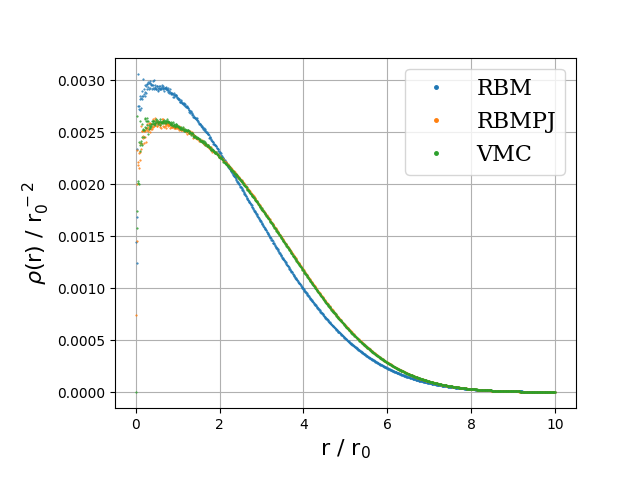
\includegraphics[width=8cm]{/home/evenmn/VMC/plots/int1/onebody/3D/2P/0.100000w/3D_2P_0p100000w_MC2pow28.png}}}
	\subfloat[8P, $\omega=0.1$]{{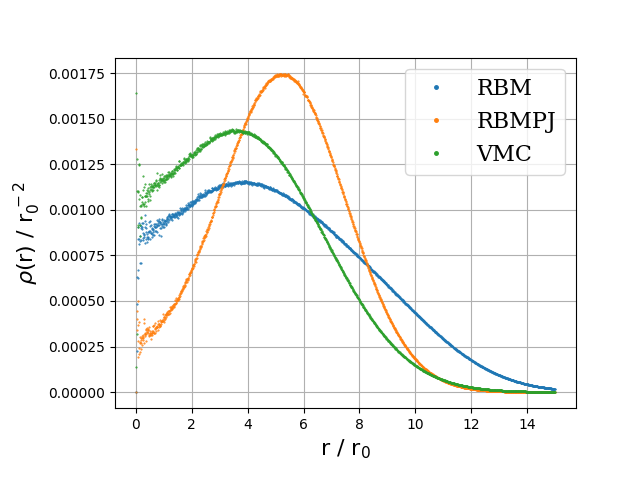
\includegraphics[width=8cm]{/home/evenmn/VMC/plots/int1/onebody/3D/8P/0.100000w/3D_8P_0p100000w_MC2pow28.png}}}\\
	
	\subfloat[2P, $\omega=0.5$]{{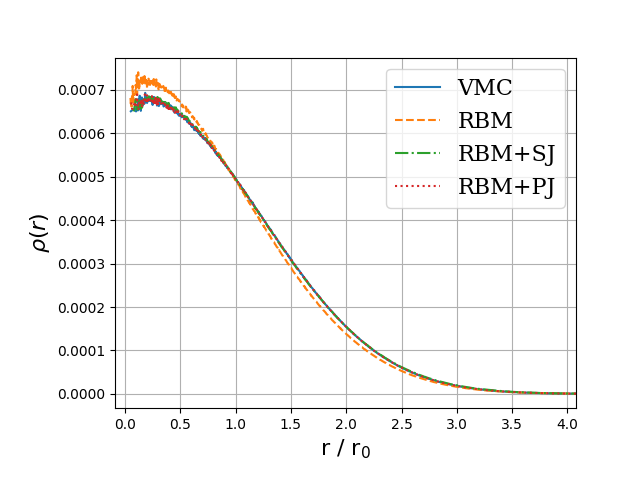
\includegraphics[width=8cm]{/home/evenmn/VMC/plots/int1/onebody/3D/2P/0.500000w/3D_2P_0p500000w_MC2pow28.png}}}
	\subfloat[8P, $\omega=0.5$]{{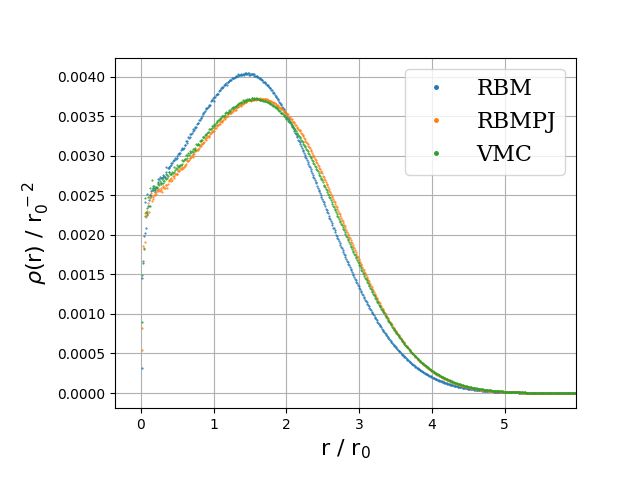
\includegraphics[width=8cm]{/home/evenmn/VMC/plots/int1/onebody/3D/8P/0.500000w/3D_8P_0p500000w_MC2pow28.png}}}\\
	
	\subfloat[2P, $\omega=1.0$]{{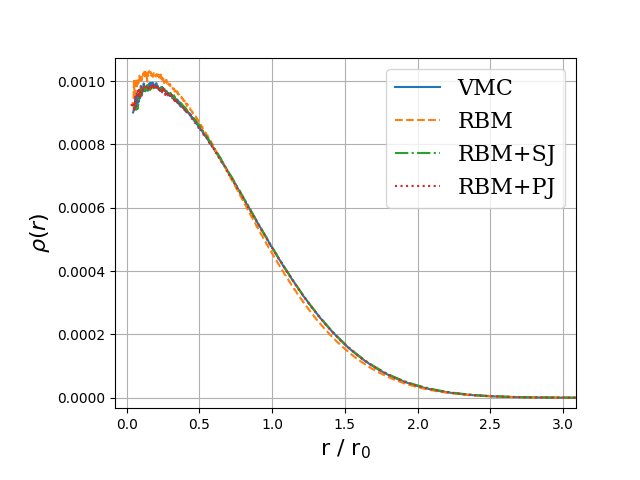
\includegraphics[width=8cm]{/home/evenmn/VMC/plots/int1/onebody/3D/2P/1.000000w/3D_2P_1p000000w_MC2pow28.png}}}
	\subfloat[8P, $\omega=1.0$]{{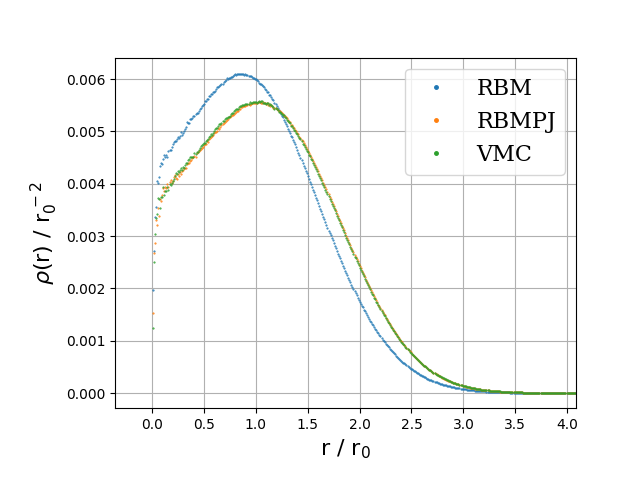
\includegraphics[width=8cm]{/home/evenmn/VMC/plots/int1/onebody/3D/8P/1.000000w/3D_8P_1p000000w_MC2pow28.png}}}
	
	%\caption{One-body densities of two and eight interacting electrons in three dimensions for various oscillator frequencies produced by standard variational Monte-Carlo (VMC), plain restricted Boltzmann machine (RBM) and restricted Boltzmann machine with Padé-Jastrow factor (RBMPJ). Stochastic gradient descent was used, and after convergence the number of Monte-Carlo cycles was $MC=2^{28}=268.435.456$.}%
	%\label{fig:OB_interaction_2P_3D}
\end{figure}
\begin{figure} [H]%
	\centering
	\subfloat[2P, $\omega=0.1$]{{\includegraphics[width=8cm]{/home/evenmn/VMC/plots/int1/onebody/3D/20P/0.100000w/ADAM_MC2pow28.png}}}
	\subfloat[8P, $\omega=0.1$]{{\includegraphics[width=8cm]{/home/evenmn/VMC/plots/int1/onebody/3D/40P/0.100000w/ADAM_MC2pow28.png}}}\\
	
	\subfloat[2P, $\omega=0.5$]{{\includegraphics[width=8cm]{/home/evenmn/VMC/plots/int1/onebody/3D/20P/0.500000w/ADAM_MC2pow28.png}}}
	\subfloat[8P, $\omega=0.5$]{{\includegraphics[width=8cm]{/home/evenmn/VMC/plots/int1/onebody/3D/40P/0.500000w/ADAM_MC2pow28.png}}}\\
	
	\subfloat[2P, $\omega=1.0$]{{\includegraphics[width=8cm]{/home/evenmn/VMC/plots/int1/onebody/3D/20P/1.000000w/ADAM_MC2pow28.png}}}
	\subfloat[8P, $\omega=1.0$]{{\includegraphics[width=8cm]{/home/evenmn/VMC/plots/int1/onebody/3D/40P/1.000000w/ADAM_MC2pow28.png}}}
	
	\caption{One-body density plots for three-dimensional circular quantum dots of 2, 8, 20 and 40 interacting electrons for various oscillator frequencies $\omega$ produced by standard variational Monte-Carlo (VMC), plain restricted Boltzmann machine (RBM), restricted Boltzmann machine with simple Jastrow factor (RBM+SJ) and restricted Boltzmann machine with Padé-Jastrow factor (RBM+PJ). ADAM optimizer was used, and after convergence the number of Monte-Carlo cycles was $MC=2^{28}=268,435,456$.}%
	\label{fig:OB_interaction_3D}
\end{figure}

\subsection{Two-body density}
The last thing we will investigate, is the two-body density. See figure \eqref{fig:TB_interaction_2D}.

\begin{landscape}
	\begin{figure} [H]%
		\centering
		\subfloat[RBM, 2P]{{\includegraphics[width=5cm]{/home/evenmn/VMC/plots/int1/twobody/2D/2P/1.000000w/RBM_ADAM_MC2pow28.png}}}
		\subfloat[RBM+SJ, 2P]{{\includegraphics[width=5cm]{/home/evenmn/VMC/plots/int1/twobody/2D/2P/1.000000w/RBMSJ_ADAM_MC2pow28.png}}}
		\subfloat[RBM+PJ, 2P]{{\includegraphics[width=5cm]{/home/evenmn/VMC/plots/int1/twobody/2D/2P/1.000000w/RBMPJ_ADAM_MC2pow28.png}}}
		\subfloat[VMC, 2P]{{\includegraphics[width=5cm]{/home/evenmn/VMC/plots/int1/twobody/2D/2P/1.000000w/VMC_ADAM_MC2pow28.png}}}\\
		
		\subfloat[RBM, 6P]{{\includegraphics[width=5cm]{/home/evenmn/VMC/plots/int1/twobody/2D/6P/1.000000w/RBM_ADAM_MC2pow28.png}}}
		\subfloat[RBM+SJ, 6P]{{\includegraphics[width=5cm]{/home/evenmn/VMC/plots/int1/twobody/2D/6P/1.000000w/RBMSJ_ADAM_MC2pow28.png}}}
		\subfloat[RBM+PJ, 6P]{{\includegraphics[width=5cm]{/home/evenmn/VMC/plots/int1/twobody/2D/6P/1.000000w/RBMPJ_ADAM_MC2pow28.png}}}
		\subfloat[VMC, 6P]{{\includegraphics[width=5cm]{/home/evenmn/VMC/plots/int1/twobody/2D/6P/1.000000w/VMC_ADAM_MC2pow28.png}}}\\
		
		\subfloat[RBM, 12P]{{\includegraphics[width=5cm]{/home/evenmn/VMC/plots/int1/twobody/2D/12P/1.000000w/RBM_ADAM_MC2pow28.png}}}
		\subfloat[RBM+SJ, 12P]{{\includegraphics[width=5cm]{/home/evenmn/VMC/plots/int1/twobody/2D/12P/1.000000w/RBMSJ_ADAM_MC2pow28.png}}}
		\subfloat[RBM+PJ, 12P]{{\includegraphics[width=5cm]{/home/evenmn/VMC/plots/int1/twobody/2D/12P/1.000000w/RBMPJ_ADAM_MC2pow28.png}}}
		\subfloat[VMC, 12P]{{\includegraphics[width=5cm]{/home/evenmn/VMC/plots/int1/twobody/2D/12P/1.000000w/VMC_ADAM_MC2pow28.png}}}\\
		
		%\caption{Two-body densities for interacting electrons in two dimensions for $\omega=0.5$ produced by standard variational Monte-Carlo (VMC), plain restricted Boltzmann machine (RBM) and restricted Boltzmann machine with Padé-Jastrow factor (RBMPJ). ADAM optimizer was used, and after convergence the number of Monte-Carlo cycles was $MC=2^{28}=268.435.456$.}%
		%\label{fig:TB_interaction_2D_1}
	\end{figure}
	
	\begin{figure} [H]%
		\centering
		\subfloat[RBM, 20P]{{\includegraphics[width=5cm]{/home/evenmn/VMC/plots/int1/twobody/2D/20P/1.000000w/RBM_ADAM_MC2pow28.png}}}
		\subfloat[RBM+SJ, 20P]{{\includegraphics[width=5cm]{/home/evenmn/VMC/plots/int1/twobody/2D/20P/1.000000w/RBMSJ_ADAM_MC2pow28.png}}}
		\subfloat[RBM+PJ, 20P]{{\includegraphics[width=5cm]{/home/evenmn/VMC/plots/int1/twobody/2D/20P/1.000000w/RBMPJ_ADAM_MC2pow28.png}}}
		\subfloat[VMC, 20P]{{\includegraphics[width=5cm]{/home/evenmn/VMC/plots/int1/twobody/2D/20P/1.000000w/VMC_ADAM_MC2pow28.png}}}
		
		\subfloat[RBM, 30P]{{\includegraphics[width=5cm]{/home/evenmn/VMC/plots/int1/twobody/2D/30P/1.000000w/RBM_ADAM_MC2pow28.png}}}
		\subfloat[RBM+SJ, 30P]{{\includegraphics[width=5cm]{/home/evenmn/VMC/plots/int1/twobody/2D/30P/1.000000w/RBMSJ_ADAM_MC2pow28.png}}}
		\subfloat[RBM+PJ, 30P]{{\includegraphics[width=5cm]{/home/evenmn/VMC/plots/int1/twobody/2D/30P/1.000000w/RBMPJ_ADAM_MC2pow28.png}}}
		%\subfloat[RBM+PJ, 30P]{{\includegraphics[width=4cm]{Images/example.png}}}
		\subfloat[VMC, 30P]{{\includegraphics[width=5cm]{/home/evenmn/VMC/plots/int1/twobody/2D/30P/1.000000w/VMC_ADAM_MC2pow28.png}}}\\
		
		\subfloat[RBM, 42P]{{\includegraphics[width=5cm]{/home/evenmn/VMC/plots/int1/twobody/2D/42P/1.000000w/RBM_ADAM_MC2pow28.png}}}
		\subfloat[RBM+SJ, 42P]{{\includegraphics[width=5cm]{/home/evenmn/VMC/plots/int1/twobody/2D/42P/1.000000w/RBMSJ_ADAM_MC2pow28.png}}}
		\subfloat[RBM+PJ, 42P]{{\includegraphics[width=5cm]{/home/evenmn/VMC/plots/int1/twobody/2D/42P/1.000000w/RBMPJ_ADAM_MC2pow28.png}}}
		\subfloat[VMC, 42P]{{\includegraphics[width=5cm]{/home/evenmn/VMC/plots/int1/twobody/2D/42P/1.000000w/VMC_ADAM_MC2pow28.png}}}\\
		
		\caption{Two-body densities for two-dimensional circular quantum dots of oscillator frequency $\omega=1.0$ produced with plain restricted Boltzmann machine (RBM), restricted Boltzmann machine with simple Jastrow factor (RBM+SJ), restricted Boltzmann machine with Padé-Jastrow factor (RBM+PJ) and standard variational Monte-Carlo (VMC). ADAM optimizer was used, and after convergence the number of Monte-Carlo cycles was $MC=2^{28}=268.435.456$.}%
		\label{fig:TB_interaction_2D}
	\end{figure}
\end{landscape}
\fi

\subsection{Energy distribution}
It is also interesting to investigate how the energy is distributed between kinetic energy, external energy and interaction energy for the different methods and various oscillator frequencies. This makes us able to check if the results agree with the virial theorem presented in section \ref{sec:virial}, and it is also interesting to see if the different methods have different energy distribution. In figure \eqref{fig:energysplit}, the kinetic energy, external potential energy and interaction energy are plotted as a function of oscillator frequency for a two-dimensional quantum dot containing two electrons.  
\begin{figure}[H]  
	\centering 
	\subfloat[$\langle \mathcal{T} \rangle$]{{% This file was created by tikzplotlib v0.8.1.
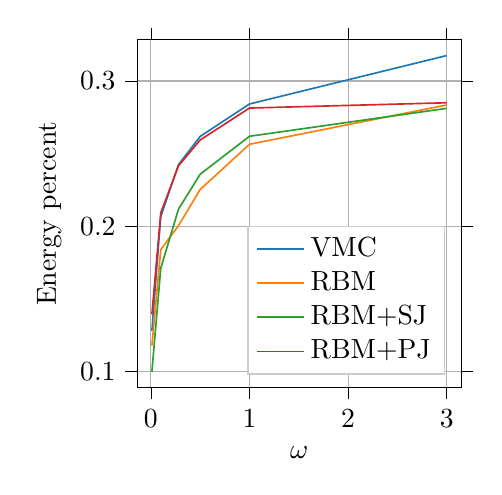
\begin{tikzpicture}

\definecolor{color0}{rgb}{0.12156862745098,0.466666666666667,0.705882352941177}
\definecolor{color1}{rgb}{1,0.498039215686275,0.0549019607843137}
\definecolor{color2}{rgb}{0.172549019607843,0.627450980392157,0.172549019607843}
\definecolor{color3}{rgb}{0.83921568627451,0.152941176470588,0.156862745098039}

\begin{axis}[
legend cell align={left},
legend style={at={(0.34,0.465)}, 
anchor=north west, 
draw=white!80.0!black},
tick align=outside,
tick pos=both,
x grid style={white!69.01960784313725!black},
xlabel={\(\displaystyle \omega\)},
xmajorgrids,
xmin=-0.1395, 
xmax=3.1495,
width=5.7cm,
height=6cm,
xtick style={color=black},
y grid style={white!69.01960784313725!black},
%ylabel={\(\displaystyle \langle\mathcal{T}\rangle/\langle\mathcal{H}\rangle\)},
ylabel={Energy percent},
ymajorgrids,
ymin=0.0886881504567312, ymax=0.328434991514478,
ytick style={color=black}
]
\addplot [semithick, color0]
table {%
0.01 0.127852031861752
0.1 0.206598835233067
0.28 0.242386879599186
0.5 0.261848241290805
1 0.284160620932466
3 0.317537407830035
};
\addlegendentry{VMC}
\addplot [semithick, color1]
table {%
0.01 0.117667696708813
0.1 0.183729236351267
0.28 0.200358629222017
0.5 0.225290229128418
1 0.25640196467047
3 0.283493955803818
};
\addlegendentry{RBM}
\addplot [semithick, color2]
table {%
0.01 0.0995857341411742
0.1 0.170962072679857
0.28 0.21171261114178
0.5 0.235774449472987
1 0.261936059864241
3 0.281159628055321
};
\addlegendentry{RBM+SJ}
\addplot [semithick, color3]
table {%
0.01 0.139123159755489
0.1 0.209150178581552
0.28 0.241565753258397
0.5 0.259394072318224
1 0.28137206888815
3 0.28501634346588
};
\addlegendentry{RBM+PJ}
\end{axis}

\end{tikzpicture}}}
	\subfloat[$\langle \mathcal{V_{\text{ext}}} \rangle$]{{% This file was created by tikzplotlib v0.8.1.
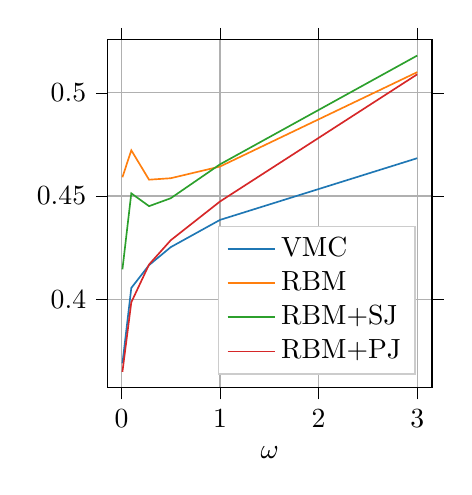
\begin{tikzpicture}

\definecolor{color0}{rgb}{0.12156862745098,0.466666666666667,0.705882352941177}
\definecolor{color1}{rgb}{1,0.498039215686275,0.0549019607843137}
\definecolor{color2}{rgb}{0.172549019607843,0.627450980392157,0.172549019607843}
\definecolor{color3}{rgb}{0.83921568627451,0.152941176470588,0.156862745098039}

\begin{axis}[
legend cell align={left},
legend style={at={(0.34,0.465)}, anchor=north west, draw=white!80.0!black},
tick align=outside,
tick pos=both,
x grid style={white!69.01960784313725!black},
xlabel={\(\displaystyle \omega\)},
xmajorgrids,
xmin=-0.1395, 
xmax=3.1495,
width=5.7cm,
height=6cm,
xtick style={color=black},
y grid style={white!69.01960784313725!black},
%ylabel={\(\displaystyle \langle\mathcal{V}_{ext}\rangle/\langle\mathcal{H}\rangle\)},
ymajorgrids,
ymin=0.357077857969547, ymax=0.525708162096253,
ytick style={color=black}
]
\addplot [semithick, color0]
table {%
0.01 0.368840286215742
0.1 0.405402343130368
0.28 0.416470956630656
0.5 0.425187077494065
1 0.438393523951776
3 0.468300433930575
};
\addlegendentry{VMC}
\addplot [semithick, color1]
table {%
0.01 0.459065945187364
0.1 0.472135608594592
0.28 0.45787868466077
0.5 0.458594258865041
1 0.464263913665448
3 0.51001255335493
};
\addlegendentry{RBM}
\addplot [semithick, color2]
table {%
0.01 0.414400798844913
0.1 0.451272747888202
0.28 0.445056515423797
0.5 0.448893342339319
1 0.465330727196777
3 0.518043148272312
};
\addlegendentry{RBM+SJ}
\addplot [semithick, color3]
table {%
0.01 0.364742871793488
0.1 0.398435285447021
0.28 0.416769439778871
0.5 0.428527443049293
1 0.447328248855592
3 0.508946881991486
};
\addlegendentry{RBM+PJ}
\end{axis}

\end{tikzpicture}}}
	\subfloat[$\langle \mathcal{V_{\text{int}}} \rangle$]{{% This file was created by tikzplotlib v0.8.1.
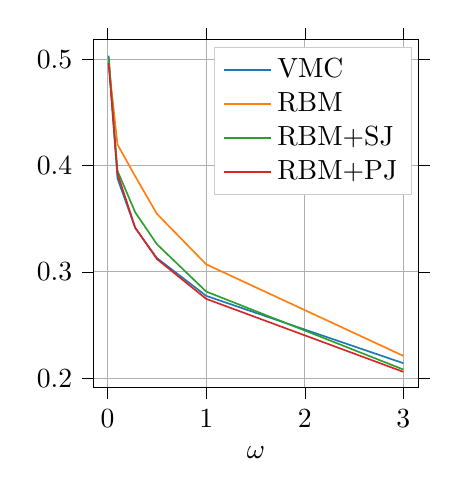
\begin{tikzpicture}

\definecolor{color0}{rgb}{0.12156862745098,0.466666666666667,0.705882352941177}
\definecolor{color1}{rgb}{1,0.498039215686275,0.0549019607843137}
\definecolor{color2}{rgb}{0.172549019607843,0.627450980392157,0.172549019607843}
\definecolor{color3}{rgb}{0.83921568627451,0.152941176470588,0.156862745098039}

\begin{axis}[
legend cell align={left},
legend style={draw=white!80.0!black},
tick align=outside,
tick pos=both,
x grid style={white!69.01960784313725!black},
xlabel={\(\displaystyle \omega\)},
xmajorgrids,
xmin=-0.1395, 
xmax=3.1495,
width=5.7cm,
height=6cm,
xtick style={color=black},
y grid style={white!69.01960784313725!black},
%ylabel={\(\displaystyle \langle\mathcal{V}_{int}\rangle/\langle\mathcal{H}\rangle\)},
ymajorgrids,
ymin=0.191165902683016, 
ymax=0.518171576172005,
ytick style={color=black}
]
\addplot [semithick, color0]
table {%
0.01 0.503307681922506
0.1 0.38793083913073
0.28 0.341220447784562
0.5 0.313000831455529
1 0.277425850848181
3 0.214161397002197
};
\addlegendentry{VMC}
\addplot [semithick, color1]
table {%
0.01 0.496579270514256
0.1 0.419751686603549
0.28 0.389852672296676
0.5 0.354535359238195
1 0.307108945331474
3 0.221025315403836
};
\addlegendentry{RBM}
\addplot [semithick, color2]
table {%
0.01 0.501706991242393
0.1 0.395033732070979
0.28 0.355986484846349
0.5 0.326035151060141
1 0.281505420579566
3 0.208224572478656
};
\addlegendentry{RBM+SJ}
\addplot [semithick, color3]
table {%
0.01 0.496174450456772
0.1 0.392403197460173
0.28 0.341598249137685
0.5 0.312056190600716
1 0.274637808471633
3 0.206029796932516
};
\addlegendentry{RBM+PJ}
\end{axis}

\end{tikzpicture}}}
	\caption{In figure (a), the kinetic energy over total energy, $\langle\mathcal{T}\rangle/\langle\mathcal{H}\rangle$, of two-dimensional quantum dots containing two electrons are plotted as a function of the oscillator frequency $\omega$. Similar plots for the external potential energy and interaction energy are found in figure (b) and (c) respectively. The methods used are standard variational Monte-Carlo (VMC), plain restricted Boltzmann machine (RBM), restricted Boltzmann machine with simple Jastrow factor (RBM+SJ) and restricted Boltzmann machine with Padé-Jastrow factor.}
	\label{fig:energysplit}
\end{figure} 

One can observe that the kinetic energy and potential energy are dominant for high frequencies, but as the frequency is decreased the interaction energy gets ever more important. At frequency $\omega=0.01$, the interaction energy actually accounts for 50\% of the energy, while the kinetic energy accounts for about 10\% of the energy. We predicted this already in section \ref{sec:wigner}.

We also see a significant difference between the methods, where the plain restricted Boltzmann machine is the one that really stands out. This is not very surprising, considering that it does not have any Jastrow factor to take care of the interactions. This apparently gives a higher interaction energy and a lower kinetic energy. 

If we now recall the virial theorem in section \ref{sec:virial}, it states that the kinetic energy is related to the potential energies in a certain way. For the interaction quantum dot system, the virial theorem reads
\begin{equation}
2\langle \mathcal{T} \rangle=2\langle \mathcal{V_{\text{ext}}} \rangle-\langle \mathcal{V_{\text{int}}} \rangle
\end{equation}
which can be verified from the energy splitting. To do this accurate, we better list up the exact energies, which is done in tables \eqref{tab:splitfrequencyQD2D},\eqref{tab:splitfrequencyQD3D2P} for some selected frequencies for quantum dots containing two electrons in two- and three dimensions respectively. By doing the math, we see that the virial theorem is satisfied for low frequencies, but as the frequency increases the theorem gets more and more off. This is the case for all the methods.

\begin{table}
	\caption{This table shows how the total energy ($\langle\mathcal{H}\rangle$) is distributed between kinetic energy ($\langle\mathcal{T}\rangle$), external potential energy ($\langle\mathcal{V}_{\text{ext}}\rangle$) and interaction energy ($\langle\mathcal{V}_{\text{int}}\rangle$) of two-dimensional circular quantum dots at a wide range of frequencies $\omega$ and two interacting electrons. The methods used are standard variational Monte-Carlo (VMC), plain restricted Boltzmann machine (RBM), restricted Boltzmann machine with a simple Jastrow factor (RBM+SJ) and restricted Boltzmann machine with Padé-Jastrow factor. The energy is given in units of $\hbar$, and the numbers in parenthesis are the statistical uncertainties in the last digit.}
	\label{tab:splitfrequencyQD2D}
	\begin{tabularx}{\textwidth}{R{1cm}rrcR{2.3cm}R{2.3cm}R{2.3cm}R{2.3cm}R{0.3cm}} \hline\hline
		&\makecell{\\ \phantom{$N$} \\ \phantom{=}} & $\omega$ && \multicolumn{1}{c}{$\langle \mathcal{H}\rangle$} & \multicolumn{1}{c}{$\langle \mathcal{T}\rangle$} & \multicolumn{1}{c}{$\langle \mathcal{V_{\text{ext}}} \rangle$} & \multicolumn{1}{c}{$\langle \mathcal{V_{\text{int}}} \rangle$} \\ \hline \\
		&RBM & 0.01 && 0.07954(7) & 0.00872(2) & 0.03402(9) & 0.0368(1) \\
		%&& 0.1 && 0.4743(1) & 0.08102(8) & 0.2082(2) & 0.1851(2) \\
		%&& 0.28 && 1.0707(2) & 0.2047(1) & 0.4678(3) & 0.3983(3) \\
		&& 0.5 && 1.7234(2) & 0.3739(2) & 0.7611(3) & 0.5884(3)\\
		%&& 1.0 && 3.0829(2) & 0.7691(2) & 1.3926(4) & 0.9212(3)\\
		&& 3.0 && 7.9968(4) & 2.2346(5) & 4.0201(7) & 1.7422(4) \\ \hdashline \\
		
		&RBM+SJ & 0.01 && 0.075267(3) & 0.00738(2) & 0.03071(8) & 0.03718(8) \\
		%&& 0.1 && 0.44858(6) & 0.07539(8) & 0.1990(2) & 0.1742(1) \\
		%&& 0.28 && 1.03470(7) & 0.2163(1) & 0.4547(2) & 0.3637(2) \\
		&& 0.5 && 1.67739(9) & 0.3913(2) & 0.7450(3) & 0.5411(2)\\
		%&& 1.0 && 3.0259(1) & 0.7857(3) & 1.3958(4) & 0.8444(3)\\
		&& 3.0 && 7.9409(1) & 2.2162(5) & 4.0834(7) & 1.6413(3) \\ \hdashline \\
		
		&RBM+PJ & 0.01 && 0.074107(8) & 0.01031(3) & 0.02703(4) & 0.03677(3) \\
		%&& 0.1 && 0.440975(8) & 0.09223(9) & 0.1757(1) & 0.17304(9) \\
		%&& 0.28 && 1.021668(7) & 0.2468(1) & 0.4258(2) & 0.3490(1) \\
		&& 0.5 && 1.659637(6) & 0.4305(2) & 0.7112(2) & 0.5179(2)\\
		%&& 1.0 && 2.999587(5) & 0.8440(3) & 1.3418(3) & 0.8238(2)\\
		&& 3.0 && 7.882355(8) & 2.2466(6) & 4.0117(6) & 1.6240(3) \\ \hdashline \\
		
		&VMC & 0.01 && 0.074070(8) & 0.00947(3) & 0.02732(5) & 0.03728(4) \\
		%&& 0.1 && 0.44129(1) & 0.09117(9) & 0.1789(1) & 0.17119(9) \\
		%&& 0.28 && 1.02192(1) & 0.2477(1) & 0.4256(2) & 0.3487(1) \\
		&& 0.5 && 1.65974(1) & 0.4346(2) & 0.7057(2) & 0.5195(2) & \\
		%&& 1.0 && 2.99936(1) & 0.8523(3) & 1.3149(3) & 0.8321(2)\\
		&& 3.0 && 7.881906(9) & 2.5028(5) & 3.6911(6) & 1.6880(3) \\ \hdashline \\
	\end{tabularx}
\end{table} 
\iffalse
\begin{table}
	\caption{This table shows how the total energy ($\langle\mathcal{H}\rangle$) is distributed between kinetic energy ($\langle\mathcal{T}\rangle$), external potential energy ($\langle\mathcal{V}_{\text{ext}}\rangle$) and interaction energy ($\langle\mathcal{V}_{\text{int}}\rangle$) of two-dimensional circular quantum dots at a wide range of frequencies $\omega$ and 20 interacting electrons. The methods used are standard variational Monte-Carlo (VMC), plain restricted Boltzmann machine (RBM), restricted Boltzmann machine with a simple Jastrow factor (RBM+SJ) and restricted Boltzmann machine with Padé-Jastrow factor. The energy is given in units of $\hbar$, and the numbers in parenthesis are the statistical uncertainties in the last digit.}
	\label{tab:splitfrequencyQD2D20P}
	\begin{tabularx}{\textwidth}{R{1cm}rrcR{2.3cm}R{2.3cm}R{2.3cm}R{2.3cm}R{0.3cm}} \hline\hline
		&\makecell{\\ \phantom{$N$} \\ \phantom{=}} & $\omega$ && \multicolumn{1}{c}{$\langle \mathcal{H}\rangle$} & \multicolumn{1}{c}{$\langle \mathcal{T}\rangle$} & \multicolumn{1}{c}{$\langle \mathcal{V_{\text{ext}}} \rangle$} & \multicolumn{1}{c}{$\langle \mathcal{V_{\text{int}}} \rangle$} \\ \hline \\
		&RBM & 0.01 && - & - & - & - \\
		&& 0.5 && 96.491(4) & 8.144(3) & 34.953(8) & 53.394(8) \\
		&& 3.0 && - & - & - & - \\ \hdashline \\
		
		&RBM+SJ & 0.01 && - & - & - & - \\
		&& 0.5 && - & - & - & - \\
		&& 3.0 && - & - & - & - \\ \hdashline \\
		
		&RBM+PJ & 0.01 && - & - & - & - \\
		&& 0.5 && - & - & - & - \\
		&& 3.0 && - & - & - & - \\ \hdashline \\
		
		&VMC & 0.01 && 6.342(1) & 0.0559(2) & 2.125(6) & 4.161(6) \\
		&& 0.5 && 94.0433(9) & 7.823(3) & 33.938(6) & 52.282(5) \\
		&& 3.0 && 357.1(3) & 6(15) & 194(15) & 156.751(9) \\ \hline \hline
	\end{tabularx}
\end{table} 
\fi

\begin{table}
	\caption{This table shows how the total energy ($\langle\mathcal{H}\rangle$) is distributed between kinetic energy ($\langle\mathcal{T}\rangle$), external potential energy ($\langle\mathcal{V}_{\text{ext}}\rangle$) and interaction energy ($\langle\mathcal{V}_{\text{int}}\rangle$) of three-dimensional circular quantum dots at a wide range of frequencies $\omega$ and two interacting electrons. The methods used are standard variational Monte-Carlo (VMC), plain restricted Boltzmann machine (RBM), restricted Boltzmann machine with a simple Jastrow factor (RBM+SJ) and restricted Boltzmann machine with Padé-Jastrow factor. The energy is given in units of $\hbar$, and the numbers in parenthesis are the statistical uncertainties in the last digit.}
	\label{tab:splitfrequencyQD3D2P}
	\begin{tabularx}{\textwidth}{R{1cm}rrcR{2.3cm}R{2.3cm}R{2.3cm}R{2.3cm}R{0.3cm}} \hline\hline
		&\makecell{\\ \phantom{$N$} \\ \phantom{=}} & $\omega$ && \multicolumn{1}{c}{$\langle \mathcal{H}\rangle$} & \multicolumn{1}{c}{$\langle \mathcal{T}\rangle$} & \multicolumn{1}{c}{$\langle \mathcal{V_{\text{ext}}} \rangle$} & \multicolumn{1}{c}{$\langle \mathcal{V_{\text{int}}} \rangle$} \\ \hline \\
		&RBM & 0.01 && - & - & - & - \\
		&& 0.5 && 2.0269(1) & 0.6595(3) & 0.8778(4) & 0.4896(2) \\
		&& 3.0 && - & - & - & - \\ \hdashline \\
		
		&RBM+SJ & 0.01 && 0.07994(2) & 0.01069(3) & 0.03190(8) & 0.03735(8) \\
		&& 0.5 && 2.00371(4) & 0.6340(3) & 0.9201(4) & 0.4496(2) \\
		&& 3.0 && 10.32289(5) & 3.5281(8) & 5.6147(9) & 1.1801(2) \\ \hdashline \\
		
		&RBM+PJ & 0.01 && 0.079312(6) & 0.01283(4) & 0.02987(6) & 0.03661(4) \\
		&& 0.5 && 1.999912(5) & 0.6515(3) & 0.9040(3) & 0.4444(1) \\
		&& 3.0 && 10.31271(4) & 3.5410(8) & 5.5989(9) & 1.1728(2) \\ \hdashline \\
		
		&VMC & 0.01 && 0.079284(6) & 0.01221(4) & 0.039757(6) & 0.036319(4) \\
		&& 0.5 && 1.999977(5) & 0.6517(3) & 0.9032(3) & 0.4451(1) \\
		&& 3.0 && 10.31717(1) & 3.8365(7) & 5.2770(8) & 1.2037(2) \\ \hdashline \\
	\end{tabularx}
\end{table} 

\iffalse
\begin{table}
	\caption{This table shows how the total energy ($\langle\mathcal{H}\rangle$) is distributed between kinetic energy ($\langle\mathcal{T}\rangle$), external potential energy ($\langle\mathcal{V}_{\text{ext}}\rangle$) and interaction energy ($\langle\mathcal{V}_{\text{int}}\rangle$) of three-dimensional circular quantum dots at a wide range of frequencies $\omega$ and two interacting electrons. The methods used are standard variational Monte-Carlo (VMC), plain restricted Boltzmann machine (RBM), restricted Boltzmann machine with a simple Jastrow factor (RBM+SJ) and restricted Boltzmann machine with Padé-Jastrow factor. The energy is given in units of $\hbar$, and the numbers in parenthesis are the statistical uncertainties in the last digit.}
	\label{tab:splitfrequencyQD3D20P}
	\begin{tabularx}{\textwidth}{R{1cm}rrcR{2.3cm}R{2.3cm}R{2.3cm}R{2.3cm}R{0.3cm}} \hline\hline
		&\makecell{\\ \phantom{$N$} \\ \phantom{=}} & $\omega$ && \multicolumn{1}{c}{$\langle \mathcal{H}\rangle$} & \multicolumn{1}{c}{$\langle \mathcal{T}\rangle$} & \multicolumn{1}{c}{$\langle \mathcal{V_{\text{ext}}} \rangle$} & \multicolumn{1}{c}{$\langle \mathcal{V_{\text{int}}} \rangle$} \\ \hline \\
		&RBM & 0.01 && - & - & - & - \\
		&& 0.5 && - & - & - & - \\
		&& 3.0 && - & - & - & - \\ \hdashline \\
		
		&RBM+SJ & 0.01 && 5.7778(4) & -0.3(1) & 2.26(5) & 3.8(2) \\
		&& 0.5 && 85.893(1) & 7.212(2) & 31.722(8) & 46.958(7) \\
		&& 3.0 && 333.07(6) & 53.2(5) & 138.0(5) & 141.835(9) \\ \hdashline \\
		
		&RBM+PJ & 0.01 && - & - & - & - \\
		&& 0.5 && - & - & - & - \\
		&& 3.0 && 333.027(1) & 49.3(3) & 152.1(3) & 131.618(7) \\ \hdashline \\
		
		&VMC & 0.01 && 5.809(2) & 0.0473(2) & 1.940(7) & 3.822(7) \\
		&& 0.5 && 85.7197(6) & 7.868(2) & 31.383(6) & 46.469(5) \\
		&& 3.0 && 333.38(4) & 49.0(6) & 151.3(6) & 133.091(7) \\ \hdashline \\
	\end{tabularx}
\end{table} 
\fi

\iffalse
\begin{table}
	\caption{Total energy ($\langle\mathcal{H}\rangle$), kinetic energy ($\langle\mathcal{T}\rangle$) and potential energy ($\langle\mathcal{V}\rangle$) of two-dimensional circular quantum dots at a wide range of frequencies $\omega$. A standard variational Monte-Carlo wave function is used. The energy is given in units of $\hbar$, and the numbers in parenthesis are the statistical uncertainties in the last digit.}
	\label{tab:splitfrequencyQDVMC}
	\begin{tabularx}{\textwidth}{R{1.5cm}rrcR{2.3cm}R{2.3cm}R{2.3cm}R{2.3cm}} \hline\hline
		&\makecell{\\ $N$ \\ \phantom{=}} & $\omega$ && \multicolumn{1}{c}{$\langle \mathcal{H}\rangle$} & \multicolumn{1}{c}{$\langle \mathcal{T}\rangle$} & \multicolumn{1}{c}{$\langle \mathcal{V_{\text{ext}}} \rangle$} & \multicolumn{1}{c}{$\langle \mathcal{V_{\text{int}}} \rangle$} \\ \hline \\
		&2 & 0.01 && 0.074070(8) & 0.00947(3) & 0.02732(5) & 0.03728(4) \\
		&& 0.1 && 0.44129(1) & 0.09117(9) & 0.1789(1) & 0.17119(9) \\
		&& 0.28 && 1.02192(1) & 0.2477(1) & 0.4256(2) & 0.3487(1) \\
		&& 0.5 && 1.65974(1) & 0.4346(2) & 0.7057(2) & 0.5195(2)\\
		&& 1.0 && 2.99936(1) & 0.8523(3) & 1.3149(3) & 0.8321(2)\\
		&& 3.0 && 7.881906(9) & 2.5028(5) & 3.6911(6) & 1.6880(3) \\ \hdashline \\
		
		&6 & 0.01 && 0.6982(1) & 0.02735(7) & 0.2427(3) & 0.4281(3) \\
		&& 0.1 && 3.5695(1) & 0.3201(3) & 1.2934(6) & 1.9560(5) \\
		&& 0.28 && 7.6219(1) & 0.9105(4) & 2.8821(9) & 3.8292(7) \\
		&& 0.5 && 11.8104(2) & 1.6710(7) & 4.535(1) & 5.6045(9)\\
		&& 1.0 && 20.1918(2) & 3.405(1) & 8.046(1) & 8.741(1)\\
		&& 3.0 && 51.072(6) & 8.71(3) & 28.24(4) & 14.11(1) \\ \hdashline \\
		
		&12 & 0.01 && 2.4972(3) & 0.05506(2) & 0.858(1) & 1.584(1)\\
		&& 0.1 && 12.3196(3) & 0.6885(6) & 4.393(2) & 7.238(2) \\
		&& 0.28 && 25.7049(4) & 2.090(1) & 9.355(2) & 14.260(2) \\
		&& 0.5 && 39.2421(5) & 3.939(2) & 14.564(3) & 20.739(3) \\
		&& 1.0 && 65.7928(5) & 8.536(3) & 24.874(4) & 32.383(3) \\
		&& 3.0 && 155.5235(1) & 23(1) & 63(1) & 68.4(2) \\ \hdashline \\
		
		&20 & 0.01 && 6.342(1) & 0.0559(2) & 2.125(6) & 4.161(6) \\
		&& 0.1 && 30.086(1) & 1.243(1) & 10.587(4) & 18.257(4) \\
		&& 0.28 && 62.0755(7) & 3.902(2) & 22.228(5) & 35.946(4) \\
		&& 0.5 && 94.0433(9) & 7.823(3) & 33.938(6) & 52.282(5) \\
		&& 1.0 && 156.102(1) & 16.86(1) & 58.14(1) & 81.098(6) \\
		&& 3.0 && 357.1(3) & 6(15) & 194(15) & 156.751(9) \\ \hline \hline
	\end{tabularx}
\end{table} 

\begin{table}
	\caption{Total energy ($\langle\mathcal{H}\rangle$), kinetic energy ($\langle\mathcal{T}\rangle$) and potential energy ($\langle\mathcal{V}\rangle$) of two-dimensional circular quantum dots at a wide range of frequencies $\omega$. A plain restricted Boltzmann machine wave function is used. The energy is given in units of $\hbar$, and the numbers in parenthesis are the statistical uncertainties in the last digit.}
	\label{tab:splitfrequencyQDRBM}
	\begin{tabularx}{\textwidth}{R{1.5cm}rrcR{2.3cm}R{2.3cm}R{2.3cm}R{2.3cm}} \hline\hline
		&\makecell{\\ $N$ \\ \phantom{=}} & $\omega$ && \multicolumn{1}{c}{$\langle \mathcal{H}\rangle$} & \multicolumn{1}{c}{$\langle \mathcal{T}\rangle$} & \multicolumn{1}{c}{$\langle \mathcal{V_{\text{ext}}} \rangle$} & \multicolumn{1}{c}{$\langle \mathcal{V_{\text{int}}} \rangle$} \\ \hline \\
		&2 & 0.01 && 0.07954(7) & 0.00872(2) & 0.03402(9) & 0.0368(1) \\
		&& 0.1 && 0.4743(1) & 0.08102(8) & 0.2082(2) & 0.1851(2) \\
		&& 0.28 && 1.0707(2) & 0.2047(1) & 0.4678(3) & 0.3983(3) \\
		&& 0.5 && 1.7234(2) & 0.3739(2) & 0.7611(3) & 0.5884(3)\\
		&& 1.0 && 3.0829(2) & 0.7691(2) & 1.3926(4) & 0.9212(3)\\
		&& 3.0 && 7.9968(4) & 2.2346(5) & 4.0201(7) & 1.7422(4) \\ \hdashline \\
		
		&6 & 0.01 && 0.929(7) & -0.39(2) & 1.00(2) & 0.316(9) \\
		&& 0.1 && 3.75(1) & -0.01(4) & 1.87(4) & 1.90(2) \\
		&& 0.28 && 7.9273(9) & 0.8684(6) & 3.009(1) & 4.050(2) \\
		&& 0.5 && 12.241(1) & 1.611(1) & 4.709(2) & 5.921(2)\\
		&& 1.0 && 20.716(1) & 3.391(1) & 7.914(3) & 9.411(2)\\
		&& 3.0 && 49.415(1) & 10.309(3) & 21.456(4) & 17.649(2) \\ \hdashline \\
		
		&12 & 0.01 && - & - & - & - \\
		&& 0.1 && - & - & - & - \\
		&& 0.28 && - & - & - & - \\
		&& 0.5 && 40.442(3) & 4.116(2) & 14.868(4) & 21.458(4) \\
		&& 1.0 && 67.614(3) & 8.953(3) & 25.207(6) & 33.455(5) \\
		&& 3.0 && TIME & - & - & - \\ \hdashline \\
		
		&20 & 0.01 && EXPL & - & - & - \\
		&& 0.1 && EXPL & - & - & - \\
		&& 0.28 && TIME & - & - & - \\
		&& 0.5 && 96.491(4) & 8.144(3) & 34.953(8) & 53.394(8) \\
		&& 1.0 && 159.645(5) & 17.12(5) & 58.74(5) & 83.397(9) \\
		&& 3.0 && TIME & - & - & - \\ \hline \hline
	\end{tabularx}
\end{table} 

\begin{table}
	\caption{Total energy ($\langle\mathcal{H}\rangle$), kinetic energy ($\langle\mathcal{T}\rangle$) and potential energy ($\langle\mathcal{V}\rangle$) of two-dimensional circular quantum dots at a wide range of frequencies $\omega$. A restricted Boltzmann machine with Padé-Jastrow wave function is used. The energy is given in units of $\hbar$, and the numbers in parenthesis are the statistical uncertainties in the last digit.}
	\label{tab:splitfrequencyQDRBMPJ}
	\begin{tabularx}{\textwidth}{R{1.5cm}rrcR{2.3cm}R{2.3cm}R{2.3cm}R{2.3cm}} \hline\hline
		&\makecell{\\ $N$ \\ \phantom{=}} & $\omega$ && \multicolumn{1}{c}{$\langle \mathcal{H}\rangle$} & \multicolumn{1}{c}{$\langle \mathcal{T}\rangle$} & \multicolumn{1}{c}{$\langle \mathcal{V_{\text{ext}}} \rangle$} & \multicolumn{1}{c}{$\langle \mathcal{V_{\text{int}}} \rangle$} \\ \hline \\
		&2 & 0.01 && 0.074107(8) & 0.01031(3) & 0.02703(4) & 0.03677(3) \\
		&& 0.1 && 0.440975(8) & 0.09223(9) & 0.1757(1) & 0.17304(9) \\
		&& 0.28 && 1.021668(7) & 0.2468(1) & 0.4258(2) & 0.3490(1) \\
		&& 0.5 && 1.659637(6) & 0.4305(2) & 0.7112(2) & 0.5179(2)\\
		&& 1.0 && 2.999587(5) & 0.8440(3) & 1.3418(3) & 0.8238(2)\\
		&& 3.0 && 7.882355(8) & 2.2466(6) & 4.0117(6) & 1.6240(3) \\ \hdashline \\
		
		&6 & 0.01 && 0.6932(5) & 0.031(2) & 0.260(2) & 0.401(1) \\
		&& 0.1 && 3.5700(2) & 0.3494(3) & 1.2805(9) & 1.9401(8) \\
		&& 0.28 && 7.6203(2) & 0.9519(6) & 2.82(1) & 3.84(1) \\
		&& 0.5 && 11.8074(2) & 1.7018(7) & 4.513(1) & 5.5927(9) \\
		&& 1.0 && 20.1832(1) & 3.428(1) & 8.068(1) & 8.687(1) \\
		&& 3.0 && 48.9157(8) & 10.789(5) & 20.383(5) & 17.743(2) \\ \hdashline \\
		
		&12 & 0.01 && 2.547(7) & 0.045(7) & 0.99(1) & 1.51(1) \\
		&& 0.1 && 12.361(1) & 0.797(1) & 4.394(3) & 7.169(3) \\
		&& 0.28 && 25.7461(6) & 2.415(1) & 9.050(2) & 14.281(2) \\
		&& 0.5 && 39.2661(6) & 4.262(2) & 14.277(2) & 20.728(2) \\
		&& 1.0 && 65.7911(5) & 8.537(3) & 25.197(4) & 32.067(3) \\
		&& 3.0 && 154.1234(7) & 23.34(7) & 70.39(7) & 60.397(4) \\ \hdashline \\
		
		&20 & 0.01 && 6.210(1) & 0.1208(5) & 2.189(2) & 3.900(2) \\
		&& 0.1 && 30.156(1) & 1.574(1) & 10.473(3) & 18.109(3) \\
		&& 0.28 && 62.210(1) & 4.657(2) & 21.227(4) & 36.106(4) \\
		&& 0.5 && 94.127(1) & 8.249(3) & 33.543(5) & 52.335(4) \\
		&& 1.0 && 156.099(1) & 16.768(6) & 58.513(8) & 80.818(6) \\
		&& 3.0 && 359.220(2) & 37.1(7) & 171.5(7) & 150.646(8) \\ \hline \hline
	\end{tabularx}
\end{table} 

\begin{table}
	\caption{Total energy ($\langle\mathcal{H}\rangle$), kinetic energy ($\langle\mathcal{T}\rangle$) and potential energy ($\langle\mathcal{V}\rangle$) of two-dimensional circular quantum dots at a wide range of frequencies $\omega$. A restricted Boltzmann machine wave function with a simple Jastrow factor is used. The energy is given in units of $\hbar$, and the numbers in parenthesis are the statistical uncertainties in the last digit.}
	\label{tab:splitfrequencyQDRBMSJ}
	\begin{tabularx}{\textwidth}{R{1.5cm}rrcR{2.3cm}R{2.3cm}R{2.3cm}R{2.3cm}} \hline\hline
		&\makecell{\\ $N$ \\ \phantom{=}} & $\omega$ && \multicolumn{1}{c}{$\langle \mathcal{H}\rangle$} & \multicolumn{1}{c}{$\langle \mathcal{T}\rangle$} & \multicolumn{1}{c}{$\langle \mathcal{V_{\text{ext}}} \rangle$} & \multicolumn{1}{c}{$\langle \mathcal{V_{\text{int}}} \rangle$} \\ \hline \\
		&2 & 0.01 && 0.075267(3) & 0.00738(2) & 0.03071(8) & 0.03718(8) \\
		&& 0.1 && 0.44858(6) & 0.07539(8) & 0.1990(2) & 0.1742(1) \\
		&& 0.28 && 1.03470(7) & 0.2163(1) & 0.4547(2) & 0.3637(2) \\
		&& 0.5 && 1.67739(9) & 0.3913(2) & 0.7450(3) & 0.5411(2)\\
		&& 1.0 && 3.0259(1) & 0.7857(3) & 1.3958(4) & 0.8444(3)\\
		&& 3.0 && 7.9409(1) & 2.2162(5) & 4.0834(7) & 1.6413(3) \\ \hdashline \\
		
		&6 & 0.01 && 0.7006(3) & 0.0376(2) & 0.2467(4) & 0.4163(4) \\
		&& 0.1 && - & - & - & - \\
		&& 0.28 && - & - & - & - \\
		&& 0.5 && - & - & - & - \\
		&& 1.0 && - & - & - & - \\
		&& 3.0 && - & - & - & - \\ \hdashline \\
		
		&12 & 0.01 && 2.4950(5) & 0.07(2) & 0.845(4) & 1.58(2) \\
		&& 0.1 && 13.11(6) & 0.29(5) & 4.8(1) & 8.1(2) \\
		&& 0.28 && 26.340(2) & 1.917(2) & 10.006(4) & 14.417(4) \\
		&& 0.5 && 41.28(1) & 4.07(1) & 16.948(5) & 20.265(4) \\
		&& 1.0 && 70.0(2) & 7.7(2) & 33.615(9) & 28.723(4) \\
		&& 3.0 && - & - & - & - \\ \hdashline \\
		
		&20 & 0.01 && 8.014(4) & 0.02(5) & 5.26(8) & 2.7(1) \\
		&& 0.1 && 30.624(3) & 1.487(2) & 10.893(5) & 18.243(5) \\
		&& 0.28 && 63.209(6) & 3.668(5) & 22.560(8) & 36.981(8) \\
		&& 0.5 && 99.917(7) & 7.574(5) & 45.20(1) & 47.144(6) \\
		&& 1.0 && 166(5) & 7(5) & 89.10(3) & 70.820(7) \\
		&& 3.0 && - & - & - & - \\ \hline \hline
	\end{tabularx}
\end{table} 

\begin{table}
	\caption{Total energy ($\langle \mathcal{H}\rangle$), kinetic energy ($\langle\mathcal{T}\rangle$) and potential energy ($\langle \mathcal{V}\rangle$) of three-dimensional circular quantum dots at a wide range of frequencies $\omega$. A restricted Boltzmann machine with Padé-Jastrow wave function is used. The energy is given in units of $\hbar$, and the numbers in parenthesis are the statistical uncertainties in the last digit.}
	\label{tab:splitfrequencyQDRBMPJ3D}
	\begin{tabularx}{\textwidth}{R{1.5cm}rrcR{2.3cm}R{2.3cm}R{2.3cm}R{2.3cm}} \hline\hline
		&\makecell{\\ $N$ \\ \phantom{=}} & $\omega$ && \multicolumn{1}{c}{$\langle \mathcal{H}\rangle$} & \multicolumn{1}{c}{$\langle \mathcal{T}\rangle$} & \multicolumn{1}{c}{$\langle \mathcal{V_{\text{ext}}} \rangle$} & \multicolumn{1}{c}{$\langle \mathcal{V_{\text{int}}} \rangle$} \\ \hline \\
		&2 & 0.01 && 0.079312(6) & 0.01283(4) & 0.02987(6) & 0.03661(4) \\
		&& 0.1 && 0.500080(6) & 0.1271(1) & 0.2085(2) & 0.1644(1) \\
		&& 0.28 && 1.201717(6) & 0.3619(2) & 0.5258(3) & 0.3140(1) \\
		&& 0.5 && 1.999912(5) & 0.6515(3) & 0.9040(3) & 0.4444(1) \\
		&& 1.0 && 3.729827(5) & 1.2995(4) & 1.7688(5) & 0.6615(2) \\
		&& 3.0 && 10.31271(4) & 3.5410(8) & 5.5989(9) & 1.1728(2) \\ \hdashline \\
		
		&8 & 0.01 && EXPL & - & - & - \\
		&& 0.1 && 5.8562(9) & 0.6134(7) & 2.088(2) & 3.155(2) \\
		&& 0.28 && 12.2056(2) & 1.5665(7) & 4.605(1) & 6.034(1) \\
		&& 0.5 && 18.9747(2) & 2.972(1) & 7.344(2) & 8.659(1) \\
		&& 1.0 && 32.6820(2) & 6.266(2) & 13.390(3) & 13.026(1) \\
		&& 3.0 && 80.6280(3) & 18.35(2) & 38.64(2) & 23.627(2) \\ \hdashline \\
		
		&20 & 0.01 && 6.012(2) & 0.156(2) & 3.00(2) & 2.860(2) \\
		&& 0.1 && 27.774(2) & 1.694(2) & 9.527(5) & 16.553(5) \\
		&& 0.28 && 57.722(4) & 5.00(7) & 20.4(1) & 32.35(5) \\
		&& 0.5 && EXPL & - & - & - \\
		&& 1.0 && TIME & - & - & - \\
		&& 3.0 && 333.027(1) & 49.3(3) & 152.1(3) & 131.618(7) \\ \hdashline \\
		
		&40 & 0.01 && - & - & - & - \\
		&& 0.1 && - & - & - & - \\
		&& 0.28 && - & - & - & - \\
		&& 0.5 && - & - & - & - \\
		&& 1.0 && - & - & - & - \\
		&& 3.0 && - & - & - & - \\ \hline \hline
	\end{tabularx}
\end{table}

\begin{table}
	\caption{Total energy ($\langle \mathcal{H}\rangle$), kinetic energy ($\langle\mathcal{T}\rangle$) and potential energy ($\langle \mathcal{V}\rangle$) of three-dimensional circular quantum dots at a wide range of frequencies $\omega$. A standard variational Monte-Carlo wave function is used. The energy is given in units of $\hbar$, and the numbers in parenthesis are the statistical uncertainties in the last digit.}
	\label{tab:splitfrequencyQDVMC3D}
	\begin{tabularx}{\textwidth}{R{1.5cm}rrcR{2.3cm}R{2.3cm}R{2.3cm}R{2.3cm}} \hline\hline
		&\makecell{\\ $N$ \\ \phantom{=}} & $\omega$ && \multicolumn{1}{c}{$\langle \mathcal{H}\rangle$} & \multicolumn{1}{c}{$\langle \mathcal{T}\rangle$} & \multicolumn{1}{c}{$\langle \mathcal{V_{\text{ext}}} \rangle$} & \multicolumn{1}{c}{$\langle \mathcal{V_{\text{int}}} \rangle$} \\ \hline \\
		&2 & 0.01 && 0.079284(6) & 0.01221(4) & 0.039757(6) & 0.036319(4) \\
		&& 0.1 && 0.500083(7) & 0.1263(1) & 0.2082(2) & 0.1656(1) \\
		&& 0.28 && 1.201752(6) & 0.3606(2) & 0.5272(3) & 0.3140(1) \\
		&& 0.5 && 1.999977(5) & 0.6517(3) & 0.9032(3) & 0.4451(1) \\
		&& 1.0 && 3.730030(5) & 1.3105(4) & 1.7551(5) & 0.6644(2) \\
		&& 3.0 && 10.31717(1) & 3.8365(7) & 5.2770(8) & 1.2037(2) \\ \hdashline \\
		
		&8 & 0.01 && 1.1490(4) & 0.02339(8) & 0.427(1) & 0.6985(9) \\
		&& 0.1 && 5.7126(1) & 0.4930(4) & 2.085(1) & 3.1342(9) \\
		&& 0.28 && 12.2050(2) & 1.5332(7) & 4.630(2) & 6.041(1) \\
		&& 0.5 && 19.03(2) & 3.14(3) & 6.62(2) & 9.27(3) \\
		&& 1.0 && 32.6863(2) & 6.244(2) & 13.378(3) & 13.064(1) \\
		&& 3.0 && 80.73(6) & 19.1(1) & 37.66(9) & 23.93(5) \\ \hdashline \\
		
		&20 & 0.01 && 5.809(2) & 0.0473(2) & 1.940(7) & 3.822(7) \\
		&& 0.1 && 27.3152(5) & 1.247(1) & 9.392(3) & 16.676(3) \\
		&& 0.28 && 56.4386(5) & 3.991(2) & 20.125(5) & 32.322(4) \\
		&& 0.5 && 85.7197(6) & 7.868(2) & 31.383(6) & 46.469(5) \\
		&& 1.0 && 142.9561(7) & 17.29(2) & 54.45(3) & 71.218(6) \\
		&& 3.0 && 333.38(4) & 49.0(6) & 151.3(6) & 133.091(7) \\ \hdashline \\
		
		&40 & 0.01 && - & - & - & - \\
		&& 0.1 && - & - & - & - \\
		&& 0.28 && - & - & - & - \\
		&& 0.5 && - & - & - & - \\
		&& 1.0 && - & - & - & - \\
		&& 3.0 && - & - & - & - \\ \hline \hline
	\end{tabularx}
\end{table}

\begin{table}
	\caption{Total energy ($\langle \mathcal{H}\rangle$), kinetic energy ($\langle\mathcal{T}\rangle$) and potential energy ($\langle \mathcal{V}\rangle$) of three-dimensional circular quantum dots at a wide range of frequencies $\omega$. A plain restricted Boltzmann machine wave function is used. The energy is given in units of $\hbar$, and the numbers in parenthesis are the statistical uncertainties in the last digit.}
	\label{tab:splitfrequencyQDRBM3D}
	\begin{tabularx}{\textwidth}{R{1.5cm}rrcR{2.3cm}R{2.3cm}R{2.3cm}R{2.3cm}} \hline\hline
		&\makecell{\\ $N$ \\ \phantom{=}} & $\omega$ && \multicolumn{1}{c}{$\langle \mathcal{H}\rangle$} & \multicolumn{1}{c}{$\langle \mathcal{T}\rangle$} & \multicolumn{1}{c}{$\langle \mathcal{V_{\text{ext}}} \rangle$} & \multicolumn{1}{c}{$\langle \mathcal{V_{\text{int}}} \rangle$} \\ \hline \\
		&2 & 0.01 && EXPL & - & - & - \\
		&& 0.1 && 0.5177(1) & 0.1249(1) & 0.2065(2) & 0.1863(2) \\
		&& 0.28 && 1.2261(1) & 0.35(2) & 0.53(2) & 0.3488(6) \\
		&& 0.5 && 2.0269(1) & 0.6595(3) & 0.8778(4) & 0.4896(2) \\
		&& 1.0 && 3.7574(1) & 1.3224(5) & 1.7215(5) & 0.7136(2) \\
		&& 3.0 && DID START & - & - & - \\ \hdashline \\
		
		&8 & 0.01 && EXPL & - & - & - \\
		&& 0.1 && EXPL & - & - & - \\
		&& 0.28 && EXPL & - & - & - \\
		&& 0.5 && EXPL & - & - & - \\
		&& 1.0 && 33.305(1) & 7.032(2) & 12.267(3) & 14.006(2) \\
		&& 3.0 && 80.677(1) & 17(3) & 38(3) & 25.0(1) \\ \hdashline \\
		
		&20 & 0.01 && EXPL & - & - & - \\
		&& 0.1 && ERROR & - & - & - \\
		&& 0.28 && EXPL & - & - & - \\
		&& 0.5 && EXPL & - & - & - \\
		&& 1.0 && 147.03(1) & 1(4) & 79(5) & 66(1) \\
		&& 3.0 && EXPL & - & - & - \\ \hdashline \\
		
		&40 & 0.01 && - & - & - & - \\
		&& 0.1 && - & - & - & - \\
		&& 0.28 && - & - & - & - \\
		&& 0.5 && - & - & - & - \\
		&& 1.0 && - & - & - & - \\
		&& 3.0 && - & - & - & - \\ \hline \hline
	\end{tabularx}
\end{table}

\begin{table}
	\caption{Total energy ($\langle \mathcal{H}\rangle$), kinetic energy ($\langle\mathcal{T}\rangle$) and potential energy ($\langle \mathcal{V}\rangle$) of three-dimensional circular quantum dots at a wide range of frequencies $\omega$. A restricted Boltzmann machine with a simple Jastrow factor is used. The energy is given in units of $\hbar$, and the numbers in parenthesis are the statistical uncertainties in the last digit.}
	\label{tab:splitfrequencyQDRBMSJ3D}
	\begin{tabularx}{\textwidth}{R{1.5cm}rrcR{2.3cm}R{2.3cm}R{2.3cm}R{2.3cm}} \hline\hline
		&\makecell{\\ $N$ \\ \phantom{=}} & $\omega$ && \multicolumn{1}{c}{$\langle \mathcal{H}\rangle$} & \multicolumn{1}{c}{$\langle \mathcal{T}\rangle$} & \multicolumn{1}{c}{$\langle \mathcal{V_{\text{ext}}} \rangle$} & \multicolumn{1}{c}{$\langle \mathcal{V_{\text{int}}} \rangle$} \\ \hline \\
		&2 & 0.01 && 0.07994(2) & 0.01069(3) & 0.03190(8) & 0.03735(8) \\
		&& 0.1 && 0.50214(3) & 0.1178(1) & 0.2177(2) & 0.1666(1) \\
		&& 0.28 && 1.20475(4) & 0.3497(2) & 0.5326(3) & 0.3225(1) \\
		&& 0.5 && 2.00371(4) & 0.6340(3) & 0.9201(4) & 0.4496(2) \\
		&& 1.0 && 3.73543(4) & 1.2801(4) & 1.7871(5) & 0.6683(2) \\
		&& 3.0 && 10.32289(5) & 3.5281(8) & 5.6147(9) & 1.1801(2) \\ \hdashline \\
		
		&8 & 0.01 && 1.1371(5) & 0.02(1) & 0.388(6) & 0.73(2) \\
		&& 0.1 && 5.7498(4) & 0.4107(3) & 2.113(1) & 3.226(1) \\
		&& 0.28 && 12.2492(4) & 1.3909(6) & 4.756(2) & 6.101(1) \\
		&& 0.5 && 19.0241(4) & 2.7417(9) & 7.579(2) & 8.704(2) \\
		&& 1.0 && EXPL & - & - & - \\
		&& 3.0 && EXPL & - & - & - \\ \hdashline \\
		
		&20 & 0.01 && 5.7778(4) & -0.3(1) & 2.26(5) & 3.8(2) \\
		&& 0.1 && 27.470(1) & 0.9593(9) & 9.711(6) & 16.800(5) \\
		&& 0.28 && 56.600(1) & 3.515(1) & 20.616(7) & 32.469(6) \\
		&& 0.5 && 85.893(1) & 7.212(2) & 31.722(8) & 46.958(7) \\
		&& 1.0 && 143.209(2) & 16.531(7) & 54.86(1) & 71.819(7) \\
		&& 3.0 && 333.07(6) & 53.2(5) & 138.0(5) & 141.835(9) \\ \hdashline \\
		
		&40 & 0.01 && - & - & - & - \\
		&& 0.1 && - & - & - & - \\
		&& 0.28 && - & - & - & - \\
		&& 0.5 && - & - & - & - \\
		&& 1.0 && - & - & - & - \\
		&& 3.0 && - & - & - & - \\ \hline \hline
	\end{tabularx}
\end{table}
\fi

\newpage
\subsection{Low frequency dots}
As we pointed out in section \ref{sec:wigner}, and as shown in the previous section, the potential energy dominates the kinetic energy as low frequencies. This means that the electrons have a lower average momentum, which makes Wigner crystallization possible. As already discussed in the theory part, this phenomenon can be observed by some distinct peaks in the one-body density plots. In figure \eqref{fig:lowfreqOB}, the one-body density is plotted for low frequency dots containing 2, 6, 12 and 20 particles. 

\begin{figure}[H]
	\centering
	\subfloat[2P]{\includegraphics[scale=0.4]{/home/evenmn/VMC/plots/int1/onebody/2D/2P/0.010000w/ADAM_MC2pow28.png}}
	\subfloat[6P]{\includegraphics[scale=0.4]{/home/evenmn/VMC/plots/int1/onebody/2D/2P/0.010000w/ADAM_MC2pow28.png}}\\
	\subfloat[12P]{\includegraphics[scale=0.4]{/home/evenmn/VMC/plots/int1/onebody/2D/2P/0.010000w/ADAM_MC2pow28.png}}
	\subfloat[20P]{\includegraphics[scale=0.4]{/home/evenmn/VMC/plots/int1/onebody/2D/2P/0.010000w/ADAM_MC2pow28.png}}
	\caption{One-body density of two-dimensional circular quantum dots. $\omega=0.01$.}
	\label{fig:lowfreqOB}
\end{figure}

For two particles, we can see that the one-body density has a peak at a distance from origin, and a local minimum in origin. This means that the probability of finding the two electrons close to each other is low, which is as expected due to the low momentum. 

\iffalse
\subsection{$S\neq0$}
When the number of particles in the quantum dot is among the magic numbers presented in equation \eqref{eq:HOclosedshell}, the ground state is guaranteed to be found at $L=S=0$. However, if we want to look at dots of other sizes, this is often not true, and we will therefore look at some cases with $S\neq 0$. We will still stick to $L=0$ and closed shell systems.

Imagine a dot of four particles with $S=1$ (three have spin up and the last has spin down). The ground state is obviously found when a spin up and a spin down particle is in the lowest energy state, and the remaining particles are in the first excited energy state. Since the lowest states and the first excited states with spin up are filled up, this is a closed shell system.

Again, our results will be benchmarked to DMC, with references Ref.\cite{pederiva_diffusion_2000} and Ref.\cite{ghosal_incipient_2007}. The former reference also presents Hartree-Fock results which we also will use. 

The results are listed in table \eqref{tab:sneq0}, where we use a restricted Boltzmann machine with Padé-Jastrow factor (RBM+PJ) and standard variational Monte-Carlo (VMC). 

We find both the RBM+PJ and VMC to reproduce the reference energy in all the cases. 

\begin{table}
	\caption{The ground state energy of two-dimensional circular quantum dots of frequency $\omega$ for a given spin configuration ($L$,$S$). The results were obtained by a restricted Boltzmann machine with Padé-Jastrow factor (RBM+PJ) and standard variational Monte-Carlo (VMC). For reference, the Hartree-Fock limit results from Ref.\cite{pederiva_diffusion_2000} (HF) and diffusion Monte-Carlo results from Refs.\cite{pederiva_diffusion_2000},\cite{ghosal_incipient_2007} (DMC) are listed. All energies are given in units of $\hbar$, and the numbers in parenthesis are the statistical uncertainties in the last digit.}
	\label{tab:sneq0}
	\begin{tabularx}{\textwidth}{rrXrrXR{2.3cm}R{2.3cm}R{2.3cm}R{2.3cm}} \hline\hline
		\makecell{\\ $N$ \\ \phantom{=}} & \makecell{$\omega$} & \phantom{R} & $L$ & $S$ & \phantom{R} & \multicolumn{1}{c}{RBM+PJ} & \multicolumn{1}{c}{VMC} & \multicolumn{1}{c}{\makecell{HF\\ (Ref.\cite{pederiva_diffusion_2000})}} & \multicolumn{1}{c}{\makecell{DMC\\ (Ref.\cite{pederiva_diffusion_2000})$^a$\\ (Ref.\cite{ghosal_incipient_2007})$^b$}} \\ \hline \\
		4 & 0.28 && 0 & 1 && 3.7475(2) & 3.7711(5) & 3.9033 & 3.7135(3)$^a$\\ \\
		8 & 0.28 && 0 & 1 && 12.828(3) & 12.849(1) & 13.1887 & 12.6903(7)$^a$ \\
		& 0.25 && 0 & 1 && 11.807(1) & 11.852(1) & - & 11.6697(1)$^b$ \\ \\
		9 & 0.28 && 0 & 3/2 && 15.886(4) & 15.812(4) & 16.1544 & 15.4784(7)$^a$\\
		&3.0 && 0 & 3/2 && 97.164(4) & 96.936(7) & - & 97.0095(3)$^b$\\ \\
		11 & 0.28 && 0 & 1/2 && 22.285(2) & 22.252(1) & 22.8733 & 22.0750(4)$^a$ \\ \hline\hline
	\end{tabularx}
\end{table}
\fi

\subsection{Large dots}
In order to test the code, we also decided to run for systems with $N\geq 56$. This has no scientific significance, other than testing how far a VMC code can go. We look at weakly interacting particles, so we will not get any relativistic effects even when adding many particles.

\begin{table}
	\caption{Energy of large circular quantum dots, $\omega=1.0$. All energies are given in units of $\hbar$, and the numbers in parenthesis are the statistical uncertainties in the last digit.}
	\label{tab:largeQD}
	\begin{tabularx}{\textwidth}{R{0.5cm}rR{2.3cm}R{2.3cm}R{1.3cm}rR{2.3cm}R{2.3cm}} \hline\hline
		&\makecell{\\ $N$ \\ \phantom{=}} & \multicolumn{1}{c}{RBM} & \multicolumn{1}{c}{VMC} && $N$ & \multicolumn{1}{c}{RBM} & \multicolumn{1}{c}{VMC} \\ \hline \\
		&72 & - & 1340.520(7) && 70 & 1129.40(2) & 1108.950(4) \\
		&90 & - & - && 112 & - \\
		&110 & - & - &&  &  \\
		\hline \hline
	\end{tabularx}
\end{table}

\newpage
\section{Double quantum dots}
Double quantum dots are systems that are very interesting when it comes to testing the Boltzmann machines. Even though we know the wave functions for the non-interacting case, they are expansions that are computational expensive to work with.

\subsection{Ground state energy}
For the interacting case, we will use Alocias Mariadason's VMC calculations with and without a Hartree-Fock basis as a reference. In addition, Jørgen Høgberget provides a DMC energy for the case with two particles and $\omega=1.0$. All the results are given in table \eqref{tab:doubleQD}.
\begin{table}
	\caption{Double quantum dots. F is the number of functions used in the expansion.}
	\label{tab:doubleQD}
	\begin{tabularx}{\textwidth}{rrXR{2.3cm}R{2.3cm}R{2.3cm}R{2.3cm}R{2.3cm}} \hline\hline
		\makecell{\\ $N$ \\ \phantom{=}} & $\omega$ & \phantom{R} & \multicolumn{1}{c}{VMC (F=1)} & \multicolumn{1}{c}{RBM+PJ} & \multicolumn{1}{c}{\makecell{VMC (F$>$1)\\ (Ref.\cite{mariadason_quantum_2018})}} & \multicolumn{1}{c}{\makecell{VMC+HF\\ (Ref.\cite{mariadason_quantum_2018})}} & \multicolumn{1}{c}{\makecell{DMC\\ (Ref.\cite{hogberget_quantum_2013})}} \\ \hline \\
		2 & 0.1 && 0.41982(4) & 0.41939(3)\\
		& 0.28 && 0.9365(1) & 0.92618(4) \\
		& 0.5 && 1.4847(2) & 1.44004(4) \\
		& 1.0 && 2.6331(5) & 2.38342(3) & 2.42238(4) & 2.36618(4) & 2.3496(1) \\ \hline \\
		
		4 & 0.1 \\
		& 0.28 \\
		& 0.5 \\
		& 1.0 && - & - & 7.95247(4) & 7.90232(4) & - \\ \hline \\
		
		6 & 0.1 \\
		& 0.28 \\
		& 0.5 \\
		& 1.0 && - & - & 16.61419(4) & 16.55609(4) \\ \hline \\
		
		8 & 0.1 \\
		& 0.28 \\
		& 0.5 \\
		& 1.0 && - & - & \\ \hline \hline
	\end{tabularx}
\end{table}
What we observe, is that the Boltzmann machine with a Padé-Jastrow factor outperforms a Hermite expansion of 10 functions, which is surprising. The reason might be that the Boltzmann machine consists of a sum over all hidden nodes, which makes it behave similar to an expansion. However, the Boltzmann machine was then again beat by the Hermite expansion with a Hartree-Fock basis. 

\newpage
\section{Atoms}
The next set of systems we will address are the real Atoms, which have been investigated by physicists since the childhood of quantum mechanics, and for that reason we have an array of computational and experimental references to use. 

\subsection{Ground state energy}
We will still stick to closed shells, and as discussed in section \ref{sec:atomic}, this includes the noble gases and a few others. In table \eqref{tab:atomswinteraction}, the ground state energies are presented.

\begin{table}
	\caption{Energy of neutral atoms of atomic number $Z$. RBM is a single Slater determinant with a plain Boltzmann machine baked in, VMC is a standard variational Monte-Carlo Slater determinant, FCI is full configuration interaction and CCD means coupled cluster doubles. $a$ is reference to \cite{bergeson_measurement_1998}, $b$ is to \cite{kramida_compilation_1997} and $c$ is to \cite{hogberget_quantum_2013}. The energy is in units of $\hbar$.}
	\label{tab:atomswinteraction}
	\begin{tabularx}{\textwidth}{lrrR{2.35cm}R{2.35cm}R{2.35cm}R{2.35cm}R{2.35cm}} \hline\hline
		Atom & $Z$ & \makecell{\\ \phantom{=}} & \multicolumn{1}{c}{RBM+PJ} & \multicolumn{1}{c}{VMC} & \multicolumn{1}{c}{FCI} & 
		\multicolumn{1}{c}{CCD} &
		\multicolumn{1}{c}{Expt.}\\ \hline \\
		
		He & 2 && - & -2.84824(9) & -2.838648 & -2.839144 & $-2.903694^a$ \\
		Be & 4 && - & - & -14.3621 & -14.5129 & $-14.6674^b$ \\
		Ne & 10 && - & - & - & - & $-128.9383^c$ \\
		Mg & 12 && - & - & - & - & $-200.054^c$ \\
		Ar & 18 && - & - & - & - & $-527.544^c$ \\
		Zn & 30 && - & - & - & - & - \\
		Kr & 36 && - & - & - & - & $-2752.054976^c$ \\ \hline\hline
	\end{tabularx}
\end{table}

\subsection{One-body density}
\begin{figure}[H]
	\centering
	\includegraphics[scale=0.7]{/home/evenmn/VMC/plots/int1/atoms/He/ADAM_MC2pow28.png}
	\caption{One-body density of Helium.}
\end{figure}

